% report/ExpFmain000.tex
\documentclass[18pt,c]{beamer}
\makeatletter
\let\beamer@writeslidentry@miniframeson=\beamer@writeslidentry
\def\beamer@writeslidentry@miniframesoff{%
  \expandafter\beamer@ifempty\expandafter{\beamer@framestartpage}{}% does not happen normally
  {%else
    % removed \addtocontents commands
   \clearpage\beamer@notesactions%
  }
}
\newcommand*{\miniframeson}{\let\beamer@writeslidentry=\beamer@writeslidentry@miniframeson}
\newcommand*{\miniframesoff}{\let\beamer@writeslidentry=\beamer@writeslidentry@miniframesoff}
\makeatother
% yellow
\definecolor{goldenyellow}{rgb}{1.0, 0.87, 0.0}
\definecolor{electricyellow}{rgb}{1.0, 1.0, 0.0}
\definecolor{icterine}{rgb}{0.99, 0.97, 0.37}
\definecolor{flavescent}{rgb}{0.97, 0.91, 0.56}
\definecolor{lemon}{rgb}{1.0, 0.97, 0.0}
% orange
\definecolor{amber}{rgb}{1.0, 0.75, 0.0}
\definecolor{cadmiumorange}{rgb}{0.93, 0.53, 0.18}
\definecolor{internationalorange}{rgb}{1.0, 0.31, 0.0}
% red
\definecolor{ferrarired}{rgb}{1.0, 0.11, 0.0}
\definecolor{fireenginered}{rgb}{0.81, 0.09, 0.13}
\definecolor{cadmiumred}{rgb}{0.89, 0.0, 0.13}
% blue
\definecolor{ao}{rgb}{0.0, 0.5, 0.0}
\definecolor{babyblueeyes}{rgb}{0.63, 0.79, 0.95}
\definecolor{bleudefrance}{rgb}{0.19, 0.55, 0.91}
\definecolor{blue}{rgb}{0.0, 0.0, 1.0}
\definecolor{cobalt}{rgb}{0.0, 0.28, 0.67}
\definecolor{darkmidnightblue}{rgb}{0.0, 0.2, 0.4}
\definecolor{brandeisblue}{rgb}{0.0, 0.44, 1.0}
\definecolor{deepskyblue}{rgb}{0.0, 0.75, 1.0}
\definecolor{iris}{rgb}{0.35, 0.31, 0.81}
\definecolor{navyblue}{rgb}{0.0, 0.0, 0.5}
\definecolor{ultramarine}{rgb}{0.07, 0.04, 0.56}
\definecolor{electricultramarine}{rgb}{0.25, 0.0, 1.0}
% green
\definecolor{cadmiumgreen}{rgb}{0.0, 0.42, 0.24}
\definecolor{darkpastelgreen}{rgb}{0.01, 0.75, 0.24}
\usetheme{Berlin}
\usecolortheme{default}
\usefonttheme{default}
\setbeamercolor{structure}{fg=blue}
\setbeamerfont{frametitle}{size=\footnotesize}
\usepackage{graphicx}
\renewcommand{\topfraction}{1.0}
\renewcommand{\floatpagefraction}{1.0}
\begin{document}
\title{Report of Experiment ExpF. k-Symmetry: Scalability of Learning by Grammar Tuning and Language Tuning  }
\author{Andreas Geyer-Schulz}
\date{\today}
\begin{frame}
\titlepage
\end{frame}
\begin{frame}
\frametitle{Abstract}
Grammar tuning adapts the language. Language tuning adds new language elements. In this experiment we study the complexity of learning  with increasing k with a grammar with symmetric pairs and an additional function.%\end{abstract}
\end{frame}
\begin{frame}[t, allowframebreaks]
\frametitle{Contents}
\tableofcontents[subsubsectionstyle=hide]
\vfill
\end{frame}
% report/ExpFmain001.tex
\miniframeson
\section{Design of Experiment}
% report/ExpFmain002.tex
\begin{frame}
\vspace*{2mm}
\begin{block}{
Description of Experiment
}
The purpose of this computational experiment is to study
the development of {\tt Seconds} and {	t Generations} with increasing k
for the grammar T5.
 
The {\bf problem environment} is the k-symmetry problem: 
Finding a boolean expression (with and, or, and not)
which is TRUE for symmetric k-bit strings.
 
The {\bf solution method} is grammar-based genetic programming
(option {\tt algorithm="sgp"}  of {\tt xegaRun}).
The {\bf solver} used is {\tt xegaRun} from the R-package {\tt xega}.
 
The experiment consists of 11 treatments, 1 grammar for 11 problem sizes $k\in 2,\dots, 12$.
\end{block}
\end{frame}% report/ExpFmain003.tex
\begin{frame}
\frametitle{
Description of Experiment
}
The control variable in this experiment is
\begin{itemize}
\item the bit-length of the k-symmetry problem: 2 to 12.
       for grammar {\bf T5}:
\begin{enumerate}
\item With symmetric pairs.
\item And a new base function,
       the function sPair(x, y) which is implemented by
 
 sPair $<-$ function(x,y) \{OR(AND(x,y),AND(NOT(x),NOT(y)))\}
\end{enumerate}
\end{itemize}
\end{frame}% report/ExpFmain004.tex
% ExpF
% Table: Common Parameters of Experiment ExpF
% Wed May 14 17:35:45 2025
 \begin{frame}
 \fontsize{8pt}{9pt}\selectfont
 \frametitle{ Common Parameters of Experiment ExpF }
% latex table generated in R 4.4.3 by xtable 1.8-4 package
% Wed May  7 22:00:23 2025
\begin{table}[ht]
\centering
\begin{tabular}{rr}
  \hline
 & Parameter Value \\ 
  \hline
Experiment & EE \\ 
  Optimize & Minimize! \\ 
  Trials & 10 \\ 
  Algorithm & sgp \\ 
  Max.Depth.of.DTs & 7 \\ 
  Grammar & AndOrNotTuned5.txt \\ 
  Replay & 0 \\ 
  Evaluation.Method & Deterministic \\ 
  Execution.Model & MultiCore \\ 
  Verbose & 1 \\ 
  Semantics & byValue \\ 
  Report.Eval.Errors & TRUE \\ 
  Termination.Condition & AbsoluteError \\ 
  Termination.Eps & -0.1 \\ 
  Gene.Map & Bin2Dec \\ 
   \hline
\end{tabular}
\caption{Common Parameters of Experiment ExpF (Part 1)} 
\end{table}

 \label{ExpFCommonTable000.tex}  
 \end{frame}

 % Label:  \label{ExpFCommonTable000.tex}  
% report/ExpFmain005.tex
% ExpF
% Table: Common Parameters of Experiment ExpF
% Wed May 14 17:35:45 2025
 \begin{frame}
 \fontsize{8pt}{9pt}\selectfont
 \frametitle{ Common Parameters of Experiment ExpF }
% latex table generated in R 4.4.3 by xtable 1.8-4 package
% Thu May  8 20:52:19 2025
\begin{table}[ht]
\centering
\begin{tabular}{rr}
  \hline
 & Parameter Value \\ 
  \hline
Init.Gene & InitGene \\ 
  Codon.Precision & LCM \\ 
  Population.Size & 320 \\ 
  Max.Generations & 1000 \\ 
  Crossover.Rate & 0.2 \\ 
  Mutation.Rate & 0.4 \\ 
  IV.Crossover.Rate & Const \\ 
  Crossover.Rate.2 & 0.4 \\ 
  IV.Mutation.Rate & Const \\ 
  Mutation.Rate.2 & 0.8 \\ 
   \hline
\end{tabular}
\caption{Common Parameters of Experiment ExpF (Part 2)} 
\end{table}

 \label{ExpFCommonTable001.tex}  
 \end{frame}

 % Label:  \label{ExpFCommonTable001.tex}  
% report/ExpFmain006.tex
% ExpF
% Table: Parameters of Treatments of Experiment ExpF
% Wed May 14 17:35:45 2025
 \begin{frame}
 \fontsize{8pt}{9pt}\selectfont
 \frametitle{ Parameters of Treatments of Experiment ExpF }
% latex table generated in R 4.4.3 by xtable 1.8-4 package
% Wed May  7 22:00:23 2025
\begin{table}[ht]
\centering
\begin{tabular}{rrrrr}
  \hline
 & Treatment & Problem Environment & Worst Fitness & Codons \\ 
  \hline
1 & BoolT5sgp10k & 10-Symmetry Problem & -1024 & 400 \\ 
  2 & BoolT5sgp11k & 11-Symmetry Problem & -2048 & 440 \\ 
  3 & BoolT5sgp12k & 12-Symmetry Problem & -4096 & 480 \\ 
  4 & BoolT5sgp2k & 2-Symmetry Problem &    -4 &  80 \\ 
  5 & BoolT5sgp3k & 3-Symmetry Problem &    -8 & 120 \\ 
  6 & BoolT5sgp4k & 4-Symmetry Problem &   -16 & 160 \\ 
  7 & BoolT5sgp5k & 5-Symmetry Problem &   -32 & 200 \\ 
  8 & BoolT5sgp6k & 6-Symmetry Problem &   -64 & 240 \\ 
  9 & BoolT5sgp7k & 7-Symmetry Problem &  -128 & 280 \\ 
  10 & BoolT5sgp8k & 8-Symmetry Problem &  -256 & 320 \\ 
  11 & BoolT5sgp9k & 9-Symmetry Problem &  -512 & 360 \\ 
   \hline
\end{tabular}
\caption{Parameters of Treatments of Experiment ExpF} 
\end{table}

 \label{ExpFDifferentTable000.tex}  
 \end{frame}

 % Label:  \label{ExpFDifferentTable000.tex}  
% report/ExpFmain007.tex
% ExpF
% Table: The Production Table of Experiment ExpF
% Wed May 14 17:35:45 2025
 \begin{frame}
 \fontsize{8pt}{9pt}\selectfont
 \frametitle{ The Production Table of Experiment ExpF }
% latex table generated in R 4.4.3 by xtable 1.8-4 package
% Wed May  7 22:00:23 2025
\begin{table}[ht]
\centering
\begin{tabular}{rrr}
  \hline
 & LHS & RHS \\ 
  \hline
1 & $<$fe$>$ & $<$f0$>$ \\ 
  2 & $<$fe$>$ & $<$f1$>$($<$fe$>$) \\ 
  3 & $<$fe$>$ & $<$f2$>$($<$fe$>$,$<$fe$>$) \\ 
  4 & $<$f0$>$ & D1 \\ 
  5 & $<$f0$>$ & D2 \\ 
  6 & $<$f0$>$ & D3 \\ 
  7 & $<$f0$>$ & D4 \\ 
  8 & $<$f0$>$ & D5 \\ 
  9 & $<$f0$>$ & D6 \\ 
  10 & $<$f0$>$ & D7 \\ 
  11 & $<$f0$>$ & D8 \\ 
  12 & $<$f0$>$ & D9 \\ 
  13 & $<$f0$>$ & D10 \\ 
  14 & $<$fe$>$ & sPair$<$sympairs$>$ \\ 
  15 & $<$sympairs$>$ & (D1,D10) \\ 
   \hline
\end{tabular}
\caption{The Production Table of Experiment ExpF (Part 1)} 
\end{table}

 \label{ExpFGrammarTable000.tex}  
 \end{frame}

 % Label:  \label{ExpFGrammarTable000.tex}  
% report/ExpFmain008.tex
\miniframeson
\section{Exploratory Analysis}
% report/ExpFmain009.tex
\miniframeson
\subsection{Do we always find an optimal solution?}
% report/ExpFmain010.tex
% ExpF
% Table: Fitness. k=2, ... 12.
% Wed May 14 17:35:45 2025
 \begin{frame}
 \fontsize{8pt}{9pt}\selectfont
 \frametitle{ Fitness. k=2, ... 12. }
% latex table generated in R 4.4.3 by xtable 1.8-4 package
% Sat May 10 18:58:50 2025
\begin{table}[ht]
\centering
\begin{tabular}{rrrrrrrr}
  \hline
 & Treatment & Trials & Variable & min & mean & sd & max \\ 
  \hline
1 & BoolT5sgp02k &  40 & Fitness & 0.00 & 0.00 & 0.00 & 0.00 \\ 
  5 & BoolT5sgp03k &  40 & Fitness & 0.00 & 0.00 & 0.00 & 0.00 \\ 
  9 & BoolT5sgp04k &  40 & Fitness & 0.00 & 0.00 & 0.00 & 0.00 \\ 
  13 & BoolT5sgp05k &  40 & Fitness & 0.00 & 0.00 & 0.00 & 0.00 \\ 
  17 & BoolT5sgp06k &  40 & Fitness & 0.00 & 0.00 & 0.00 & 0.00 \\ 
  21 & BoolT5sgp07k &  40 & Fitness & 0.00 & 0.00 & 0.00 & 0.00 \\ 
  25 & BoolT5sgp08k &  40 & Fitness & 0.00 & 0.00 & 0.00 & 0.00 \\ 
  29 & BoolT5sgp09k &  40 & Fitness & 0.00 & 0.00 & 0.00 & 0.00 \\ 
  33 & BoolT5sgp10k &  40 & Fitness & 0.00 & 0.00 & 0.00 & 0.00 \\ 
  37 & BoolT5sgp11k &  40 & Fitness & 0.00 & 0.00 & 0.00 & 0.00 \\ 
  41 & BoolT5sgp12k &  40 & Fitness & 0.00 & 0.80 & 5.06 & 32.00 \\ 
   \hline
\end{tabular}
\caption{Fitness. k=2, ... 12.} 
\end{table}

 \label{ExpFStatsTable000.tex}  
 \end{frame}

 % Label:  \label{ExpFStatsTable000.tex}  
% report/ExpFmain011.tex
% ExpF
% Table: Seconds. k=2, ... 12.
% Wed May 14 17:35:45 2025
 \begin{frame}
 \fontsize{8pt}{9pt}\selectfont
 \frametitle{ Seconds. k=2, ... 12. }
% latex table generated in R 4.4.3 by xtable 1.8-4 package
% Sat May 10 18:58:50 2025
\begin{table}[ht]
\centering
\begin{tabular}{rrrrrrrr}
  \hline
 & Treatment & Trials & Variable & min & mean & sd & max \\ 
  \hline
2 & BoolT5sgp02k &  40 & Seconds & 0.28 & 0.43 & 0.16 & 0.97 \\ 
  6 & BoolT5sgp03k &  40 & Seconds & 0.30 & 0.46 & 0.15 & 0.84 \\ 
  10 & BoolT5sgp04k &  40 & Seconds & 0.37 & 0.55 & 0.20 & 1.08 \\ 
  14 & BoolT5sgp05k &  40 & Seconds & 0.41 & 0.64 & 0.20 & 1.28 \\ 
  18 & BoolT5sgp06k &  40 & Seconds & 0.54 & 2.59 & 1.77 & 6.32 \\ 
  22 & BoolT5sgp07k &  40 & Seconds & 0.99 & 3.97 & 3.29 & 18.66 \\ 
  26 & BoolT5sgp08k &  40 & Seconds & 3.43 & 27.82 & 23.84 & 97.55 \\ 
  30 & BoolT5sgp09k &  40 & Seconds & 1.61 & 28.24 & 17.52 & 65.63 \\ 
  34 & BoolT5sgp10k &  40 & Seconds & 34.67 & 284.52 & 238.05 & 1134.77 \\ 
  38 & BoolT5sgp11k &  40 & Seconds & 56.67 & 644.85 & 493.13 & 1832.77 \\ 
  42 & BoolT5sgp12k &  40 & Seconds & 470.98 & 4376.96 & 3895.03 & 19775.30 \\ 
   \hline
\end{tabular}
\caption{Seconds. k=2, ... 12.} 
\end{table}

 \label{ExpFStatsTable001.tex}  
 \end{frame}

 % Label:  \label{ExpFStatsTable001.tex}  
% report/ExpFmain012.tex
% ExpF
% Table: Generations. k=2, ... 12.
% Wed May 14 17:35:45 2025
 \begin{frame}
 \fontsize{8pt}{9pt}\selectfont
 \frametitle{ Generations. k=2, ... 12. }
% latex table generated in R 4.4.3 by xtable 1.8-4 package
% Sat May 10 18:58:50 2025
\begin{table}[ht]
\centering
\begin{tabular}{rrrrrrrr}
  \hline
 & Treatment & Trials & Variable & min & mean & sd & max \\ 
  \hline
3 & BoolT5sgp02k &  40 & Generations & 1.00 & 1.00 & 0.00 & 1.00 \\ 
  7 & BoolT5sgp03k &  40 & Generations & 1.00 & 1.00 & 0.00 & 1.00 \\ 
  11 & BoolT5sgp04k &  40 & Generations & 1.00 & 1.02 & 0.16 & 2.00 \\ 
  15 & BoolT5sgp05k &  40 & Generations & 1.00 & 1.00 & 0.00 & 1.00 \\ 
  19 & BoolT5sgp06k &  40 & Generations & 1.00 & 5.08 & 3.35 & 13.00 \\ 
  23 & BoolT5sgp07k &  40 & Generations & 1.00 & 5.92 & 4.83 & 28.00 \\ 
  27 & BoolT5sgp08k &  40 & Generations & 4.00 & 23.88 & 15.00 & 59.00 \\ 
  31 & BoolT5sgp09k &  40 & Generations & 1.00 & 15.97 & 8.67 & 38.00 \\ 
  35 & BoolT5sgp10k &  40 & Generations & 14.00 & 73.85 & 53.10 & 234.00 \\ 
  39 & BoolT5sgp11k &  40 & Generations & 12.00 & 87.50 & 55.35 & 195.00 \\ 
  43 & BoolT5sgp12k &  40 & Generations & 40.00 & 284.20 & 216.58 & 1000.00 \\ 
   \hline
\end{tabular}
\caption{Generations. k=2, ... 12.} 
\end{table}

 \label{ExpFStatsTable002.tex}  
 \end{frame}

 % Label:  \label{ExpFStatsTable002.tex}  
% report/ExpFmain013.tex
\begin{frame}
\frametitle{
Do we always find the optimal program?
}
\begin{itemize}
\item For grammar T5: {\bf No.} Not for the 12-symmetry problem.
\item For the the 12-symmetry problem, errors range from $0-32$ 
       with a mean of $0.80$ and a standard deviation
       of $5.06$ for $40$ trials.
\end{itemize}
\end{frame}% report/ExpFmain014.tex
\miniframeson
\subsection{How long to find an optimal solution?}
% report/ExpFmain015.tex
% ExpF
% Figure: Distribution of Time (s) for Grammar T5. 2-symmetry.
% Wed May 14 17:35:45 2025
 \begin{frame}
 \frametitle{ Distribution of Time (s) for Grammar T5. 2-symmetry. }
 \begin{center}
\includegraphics[width=0.5\textwidth, angle=-90]
{ExpFboxplottSeconds000.eps}
 \end{center}
 \label{ExpFboxplottSeconds000.eps}  
 \end{frame}

% report/ExpFmain016.tex
% ExpF
% Figure: Distribution of Time (s) for Grammar T5. 3-symmetry.
% Wed May 14 17:35:45 2025
 \begin{frame}
 \frametitle{ Distribution of Time (s) for Grammar T5. 3-symmetry. }
 \begin{center}
\includegraphics[width=0.5\textwidth, angle=-90]
{ExpFboxplottSeconds001.eps}
 \end{center}
 \label{ExpFboxplottSeconds001.eps}  
 \end{frame}

% report/ExpFmain017.tex
% ExpF
% Figure: Distribution of Time (s) for Grammar T5. 4-symmetry.
% Wed May 14 17:35:45 2025
 \begin{frame}
 \frametitle{ Distribution of Time (s) for Grammar T5. 4-symmetry. }
 \begin{center}
\includegraphics[width=0.5\textwidth, angle=-90]
{ExpFboxplottSeconds002.eps}
 \end{center}
 \label{ExpFboxplottSeconds002.eps}  
 \end{frame}

% report/ExpFmain018.tex
% ExpF
% Figure: Distribution of Time (s) for Grammar T5. 5-symmetry.
% Wed May 14 17:35:45 2025
 \begin{frame}
 \frametitle{ Distribution of Time (s) for Grammar T5. 5-symmetry. }
 \begin{center}
\includegraphics[width=0.5\textwidth, angle=-90]
{ExpFboxplottSeconds003.eps}
 \end{center}
 \label{ExpFboxplottSeconds003.eps}  
 \end{frame}

% report/ExpFmain019.tex
% ExpF
% Figure: Distribution of Time (s) for Grammar T5. 6-symmetry.
% Wed May 14 17:35:45 2025
 \begin{frame}
 \frametitle{ Distribution of Time (s) for Grammar T5. 6-symmetry. }
 \begin{center}
\includegraphics[width=0.5\textwidth, angle=-90]
{ExpFboxplottSeconds004.eps}
 \end{center}
 \label{ExpFboxplottSeconds004.eps}  
 \end{frame}

% report/ExpFmain020.tex
% ExpF
% Figure: Distribution of Time (s) for Grammar T5. 7-symmetry.
% Wed May 14 17:35:45 2025
 \begin{frame}
 \frametitle{ Distribution of Time (s) for Grammar T5. 7-symmetry. }
 \begin{center}
\includegraphics[width=0.5\textwidth, angle=-90]
{ExpFboxplottSeconds005.eps}
 \end{center}
 \label{ExpFboxplottSeconds005.eps}  
 \end{frame}

% report/ExpFmain021.tex
% ExpF
% Figure: Distribution of Time (s) for Grammar T5. 8-symmetry.
% Wed May 14 17:35:45 2025
 \begin{frame}
 \frametitle{ Distribution of Time (s) for Grammar T5. 8-symmetry. }
 \begin{center}
\includegraphics[width=0.5\textwidth, angle=-90]
{ExpFboxplottSeconds006.eps}
 \end{center}
 \label{ExpFboxplottSeconds006.eps}  
 \end{frame}

% report/ExpFmain022.tex
% ExpF
% Figure: Distribution of Time (s) for Grammar T5. 9-symmetry.
% Wed May 14 17:35:45 2025
 \begin{frame}
 \frametitle{ Distribution of Time (s) for Grammar T5. 9-symmetry. }
 \begin{center}
\includegraphics[width=0.5\textwidth, angle=-90]
{ExpFboxplottSeconds007.eps}
 \end{center}
 \label{ExpFboxplottSeconds007.eps}  
 \end{frame}

% report/ExpFmain023.tex
% ExpF
% Figure: Distribution of Time (s) for Grammar T5. 10-symmetry.
% Wed May 14 17:35:46 2025
 \begin{frame}
 \frametitle{ Distribution of Time (s) for Grammar T5. 10-symmetry. }
 \begin{center}
\includegraphics[width=0.5\textwidth, angle=-90]
{ExpFboxplottSeconds008.eps}
 \end{center}
 \label{ExpFboxplottSeconds008.eps}  
 \end{frame}

% report/ExpFmain024.tex
% ExpF
% Figure: Distribution of Time (s) for Grammar T5. 11-symmetry.
% Wed May 14 17:35:46 2025
 \begin{frame}
 \frametitle{ Distribution of Time (s) for Grammar T5. 11-symmetry. }
 \begin{center}
\includegraphics[width=0.5\textwidth, angle=-90]
{ExpFboxplottSeconds009.eps}
 \end{center}
 \label{ExpFboxplottSeconds009.eps}  
 \end{frame}

% report/ExpFmain025.tex
% ExpF
% Figure: Distribution of Time (s) for Grammar T5. 12-symmetry.
% Wed May 14 17:35:46 2025
 \begin{frame}
 \frametitle{ Distribution of Time (s) for Grammar T5. 12-symmetry. }
 \begin{center}
\includegraphics[width=0.5\textwidth, angle=-90]
{ExpFboxplottSeconds010.eps}
 \end{center}
 \label{ExpFboxplottSeconds010.eps}  
 \end{frame}

% report/ExpFmain026.tex
% ExpF
% Figure: Distribution of Number of Generations for Grammar T5. 2-symmetry.
% Wed May 14 17:35:46 2025
 \begin{frame}
 \frametitle{ Distribution of Number of Generations for Grammar T5. 2-symmetry. }
 \begin{center}
\includegraphics[width=0.5\textwidth, angle=-90]
{ExpFboxplottGenerations000.eps}
 \end{center}
 \label{ExpFboxplottGenerations000.eps}  
 \end{frame}

% report/ExpFmain027.tex
% ExpF
% Figure: Distribution of Number of Generations for Grammar T5. 3-symmetry.
% Wed May 14 17:35:46 2025
 \begin{frame}
 \frametitle{ Distribution of Number of Generations for Grammar T5. 3-symmetry. }
 \begin{center}
\includegraphics[width=0.5\textwidth, angle=-90]
{ExpFboxplottGenerations001.eps}
 \end{center}
 \label{ExpFboxplottGenerations001.eps}  
 \end{frame}

% report/ExpFmain028.tex
% ExpF
% Figure: Distribution of Number of Generations for Grammar T5. 4-symmetry.
% Wed May 14 17:35:46 2025
 \begin{frame}
 \frametitle{ Distribution of Number of Generations for Grammar T5. 4-symmetry. }
 \begin{center}
\includegraphics[width=0.5\textwidth, angle=-90]
{ExpFboxplottGenerations002.eps}
 \end{center}
 \label{ExpFboxplottGenerations002.eps}  
 \end{frame}

% report/ExpFmain029.tex
% ExpF
% Figure: Distribution of Number of Generations for Grammar T5. 5-symmetry.
% Wed May 14 17:35:46 2025
 \begin{frame}
 \frametitle{ Distribution of Number of Generations for Grammar T5. 5-symmetry. }
 \begin{center}
\includegraphics[width=0.5\textwidth, angle=-90]
{ExpFboxplottGenerations003.eps}
 \end{center}
 \label{ExpFboxplottGenerations003.eps}  
 \end{frame}

% report/ExpFmain030.tex
% ExpF
% Figure: Distribution of Number of Generations for Grammar T5. 6-symmetry.
% Wed May 14 17:35:46 2025
 \begin{frame}
 \frametitle{ Distribution of Number of Generations for Grammar T5. 6-symmetry. }
 \begin{center}
\includegraphics[width=0.5\textwidth, angle=-90]
{ExpFboxplottGenerations004.eps}
 \end{center}
 \label{ExpFboxplottGenerations004.eps}  
 \end{frame}

% report/ExpFmain031.tex
% ExpF
% Figure: Distribution of Number of Generations for Grammar T5. 7-symmetry.
% Wed May 14 17:35:46 2025
 \begin{frame}
 \frametitle{ Distribution of Number of Generations for Grammar T5. 7-symmetry. }
 \begin{center}
\includegraphics[width=0.5\textwidth, angle=-90]
{ExpFboxplottGenerations005.eps}
 \end{center}
 \label{ExpFboxplottGenerations005.eps}  
 \end{frame}

% report/ExpFmain032.tex
% ExpF
% Figure: Distribution of Number of Generations for Grammar T5. 8-symmetry.
% Wed May 14 17:35:46 2025
 \begin{frame}
 \frametitle{ Distribution of Number of Generations for Grammar T5. 8-symmetry. }
 \begin{center}
\includegraphics[width=0.5\textwidth, angle=-90]
{ExpFboxplottGenerations006.eps}
 \end{center}
 \label{ExpFboxplottGenerations006.eps}  
 \end{frame}

% report/ExpFmain033.tex
% ExpF
% Figure: Distribution of Number of Generations for Grammar T5. 9-symmetry.
% Wed May 14 17:35:46 2025
 \begin{frame}
 \frametitle{ Distribution of Number of Generations for Grammar T5. 9-symmetry. }
 \begin{center}
\includegraphics[width=0.5\textwidth, angle=-90]
{ExpFboxplottGenerations007.eps}
 \end{center}
 \label{ExpFboxplottGenerations007.eps}  
 \end{frame}

% report/ExpFmain034.tex
% ExpF
% Figure: Distribution of Number of Generations for Grammar T5. 10-symmetry.
% Wed May 14 17:35:46 2025
 \begin{frame}
 \frametitle{ Distribution of Number of Generations for Grammar T5. 10-symmetry. }
 \begin{center}
\includegraphics[width=0.5\textwidth, angle=-90]
{ExpFboxplottGenerations008.eps}
 \end{center}
 \label{ExpFboxplottGenerations008.eps}  
 \end{frame}

% report/ExpFmain035.tex
% ExpF
% Figure: Distribution of Number of Generations for Grammar T5. 11-symmetry.
% Wed May 14 17:35:46 2025
 \begin{frame}
 \frametitle{ Distribution of Number of Generations for Grammar T5. 11-symmetry. }
 \begin{center}
\includegraphics[width=0.5\textwidth, angle=-90]
{ExpFboxplottGenerations009.eps}
 \end{center}
 \label{ExpFboxplottGenerations009.eps}  
 \end{frame}

% report/ExpFmain036.tex
% ExpF
% Figure: Distribution of Number of Generations for Grammar T5. 12-symmetry.
% Wed May 14 17:35:46 2025
 \begin{frame}
 \frametitle{ Distribution of Number of Generations for Grammar T5. 12-symmetry. }
 \begin{center}
\includegraphics[width=0.5\textwidth, angle=-90]
{ExpFboxplottGenerations010.eps}
 \end{center}
 \label{ExpFboxplottGenerations010.eps}  
 \end{frame}

% report/ExpFmain037.tex
\begin{frame}
\frametitle{
How does the algorithm behave with growing k?
}
\begin{itemize}
\item The 12-symmetry problem did not find the optimum in 1 of out 40 trials
\end{itemize}
\end{frame}% report/ExpFmain038.tex
\miniframeson
\subsection{Computational Complexity?}
% report/ExpFmain039.tex
% ExpF
% Figure: Distribution of Number of Generations for Grammar T5
% Wed May 14 17:35:46 2025
 \begin{frame}
 \frametitle{ Distribution of Number of Generations for Grammar T5 }
 \begin{center}
\includegraphics[width=0.5\textwidth, angle=-90]
{ExpFboxplottGenerations011.eps}
 \end{center}
 \label{ExpFboxplottGenerations011.eps}  
 \end{frame}

% report/ExpFmain040.tex
% ExpF
% Figure: Distribution of Seconds for Grammar T5
% Wed May 14 17:35:46 2025
 \begin{frame}
 \frametitle{ Distribution of Seconds for Grammar T5 }
 \begin{center}
\includegraphics[width=0.5\textwidth, angle=-90]
{ExpFboxplottSeconds011.eps}
 \end{center}
 \label{ExpFboxplottSeconds011.eps}  
 \end{frame}

% report/ExpFmain041.tex
\begin{frame}
\frametitle{
Growth of Complexity?
}
\begin{itemize}
\item Complexity grows in steps of 2 of k.
       The 2 and 3, 4 and 5, 6 and 7, 8 and 9, 10 and 11 took 
       a similar number of generations.
{\bf Reason:}
       The 2- and 3-symmetry problem need the same boolean expression,
       but with different variables:
       For the 2-symmetry problem, D1 and D2.
       For the 3-symmetry problem, D1 and D3,
       D2 is ignored.
\item The number of generations grows slower than the time needed.
 
  {\bf Reason:} The cost of testing a boolean expression grows with $2^k$
 
\end{itemize}
\end{frame}% report/ExpFmain042.tex
\begin{frame}
\vspace*{2mm}
\begin{block}{
Further Research.
}
Integrate grammar and language tuning
into grammar-based genetic programming algorithms!
  
{\bf Mechanisms:}
\begin{itemize}
\item Automatic function definitions.
\item Make optimal solutions of small problem instances reusable.
\item Grammar evolution from frontiers of derivation trees.
\item Very few, but costly outliers in execution time. (12-symmetry: 5:30h.)
\end{itemize}
 
Testing by sampling?
\end{block}
\end{frame}% report/ExpFmain043.tex
\miniframeson
\section{A Summary}
% report/ExpFmain044.tex
% ExpF
% Table: Summary of statistics of experiment ExpF.
% Wed May 14 17:35:46 2025
 \begin{frame}
 \fontsize{8pt}{9pt}\selectfont
 \frametitle{ Summary of statistics of experiment ExpF. }
% latex table generated in R 4.4.3 by xtable 1.8-4 package
% Sat May 10 18:58:50 2025
\begin{table}[ht]
\centering
\begin{tabular}{rrrrrrrr}
  \hline
 & Treatment & Trials & Variable & min & mean & sd & max \\ 
  \hline
4 & BoolT5sgp02k &  40 & Evaluations & 400.00 & 400.00 & 0.00 & 400.00 \\ 
  8 & BoolT5sgp03k &  40 & Evaluations & 400.00 & 400.00 & 0.00 & 400.00 \\ 
  12 & BoolT5sgp04k &  40 & Evaluations & 400.00 & 410.00 & 63.25 & 800.00 \\ 
  16 & BoolT5sgp05k &  40 & Evaluations & 400.00 & 400.00 & 0.00 & 400.00 \\ 
  20 & BoolT5sgp06k &  40 & Evaluations & 400.00 & 2030.00 & 1338.62 & 5200.00 \\ 
  24 & BoolT5sgp07k &  40 & Evaluations & 400.00 & 2370.00 & 1930.88 & 11200.00 \\ 
  28 & BoolT5sgp08k &  40 & Evaluations & 1600.00 & 9550.00 & 5999.10 & 23600.00 \\ 
  32 & BoolT5sgp09k &  40 & Evaluations & 400.00 & 6390.00 & 3467.64 & 15200.00 \\ 
  36 & BoolT5sgp10k &  40 & Evaluations & 5600.00 & 29540.00 & 21239.64 & 93600.00 \\ 
  40 & BoolT5sgp11k &  40 & Evaluations & 4800.00 & 35000.00 & 22140.62 & 78000.00 \\ 
  44 & BoolT5sgp12k &  40 & Evaluations & 16000.00 & 113680.00 & 86630.47 & 400000.00 \\ 
  1 & BoolT5sgp02k &  40 & Fitness & 0.00 & 0.00 & 0.00 & 0.00 \\ 
  5 & BoolT5sgp03k &  40 & Fitness & 0.00 & 0.00 & 0.00 & 0.00 \\ 
  9 & BoolT5sgp04k &  40 & Fitness & 0.00 & 0.00 & 0.00 & 0.00 \\ 
  13 & BoolT5sgp05k &  40 & Fitness & 0.00 & 0.00 & 0.00 & 0.00 \\ 
   \hline
\end{tabular}
\caption{Summary of statistics of experiment ExpF. (Part 1)} 
\end{table}

 \label{ExpFStatsTable003.tex}  
 \end{frame}

 % Label:  \label{ExpFStatsTable003.tex}  
% report/ExpFmain045.tex
% ExpF
% Table: Summary of statistics of experiment ExpF.
% Wed May 14 17:35:46 2025
 \begin{frame}
 \fontsize{8pt}{9pt}\selectfont
 \frametitle{ Summary of statistics of experiment ExpF. }
% latex table generated in R 4.4.3 by xtable 1.8-4 package
% Wed May  7 22:00:23 2025
\begin{table}[ht]
\centering
\begin{tabular}{rrrrrrrr}
  \hline
 & Treatment & Trials & Variable & min & mean & sd & max \\ 
  \hline
17 & BoolT5sgp3k &  10 & Fitness & 0.00 & 0.00 & 0.00 & 0.00 \\ 
  21 & BoolT5sgp4k &  10 & Fitness & 0.00 & 0.00 & 0.00 & 0.00 \\ 
  25 & BoolT5sgp5k &  10 & Fitness & 0.00 & 0.00 & 0.00 & 0.00 \\ 
  29 & BoolT5sgp6k &  10 & Fitness & 0.00 & 0.00 & 0.00 & 0.00 \\ 
  33 & BoolT5sgp7k &  10 & Fitness & 0.00 & 0.00 & 0.00 & 0.00 \\ 
  37 & BoolT5sgp8k &  10 & Fitness & 0.00 & 0.00 & 0.00 & 0.00 \\ 
  41 & BoolT5sgp9k &  10 & Fitness & 0.00 & 0.00 & 0.00 & 0.00 \\ 
  3 & BoolT5sgp10k &  10 & Generations & 13.00 & 90.30 & 62.90 & 218.00 \\ 
  7 & BoolT5sgp11k &  10 & Generations & 26.00 & 88.40 & 75.74 & 281.00 \\ 
  11 & BoolT5sgp12k &  10 & Generations & 114.00 & 395.90 & 153.11 & 500.00 \\ 
  15 & BoolT5sgp2k &  10 & Generations & 1.00 & 1.00 & 0.00 & 1.00 \\ 
  19 & BoolT5sgp3k &  10 & Generations & 1.00 & 1.00 & 0.00 & 1.00 \\ 
  23 & BoolT5sgp4k &  10 & Generations & 1.00 & 1.20 & 0.63 & 3.00 \\ 
  27 & BoolT5sgp5k &  10 & Generations & 1.00 & 1.50 & 0.97 & 4.00 \\ 
  31 & BoolT5sgp6k &  10 & Generations & 3.00 & 8.60 & 6.06 & 24.00 \\ 
   \hline
\end{tabular}
\caption{Summary of statistics of experiment ExpF. (Part 2)} 
\end{table}

 \label{ExpFStatsTable004.tex}  
 \end{frame}

 % Label:  \label{ExpFStatsTable004.tex}  
% report/ExpFmain046.tex
% ExpF
% Table: Summary of statistics of experiment ExpF.
% Wed May 14 17:35:46 2025
 \begin{frame}
 \fontsize{8pt}{9pt}\selectfont
 \frametitle{ Summary of statistics of experiment ExpF. }
% latex table generated in R 4.4.3 by xtable 1.8-4 package
% Wed May  7 22:00:23 2025
\begin{table}[ht]
\centering
\begin{tabular}{rrrrrrrr}
  \hline
 & Treatment & Trials & Variable & min & mean & sd & max \\ 
  \hline
35 & BoolT5sgp7k &  10 & Generations & 1.00 & 6.40 & 3.13 & 11.00 \\ 
  39 & BoolT5sgp8k &  10 & Generations & 13.00 & 38.10 & 12.04 & 53.00 \\ 
  43 & BoolT5sgp9k &  10 & Generations & 7.00 & 23.90 & 15.91 & 65.00 \\ 
  2 & BoolT5sgp10k &  10 & Seconds & 13.13 & 126.76 & 104.94 & 367.04 \\ 
  6 & BoolT5sgp11k &  10 & Seconds & 52.10 & 214.71 & 204.00 & 732.73 \\ 
  10 & BoolT5sgp12k &  10 & Seconds & 587.79 & 2164.05 & 867.99 & 3009.62 \\ 
  14 & BoolT5sgp2k &  10 & Seconds & 0.16 & 0.19 & 0.02 & 0.24 \\ 
  18 & BoolT5sgp3k &  10 & Seconds & 0.18 & 0.20 & 0.01 & 0.21 \\ 
  22 & BoolT5sgp4k &  10 & Seconds & 0.18 & 0.24 & 0.08 & 0.46 \\ 
  26 & BoolT5sgp5k &  10 & Seconds & 0.23 & 0.35 & 0.14 & 0.68 \\ 
  30 & BoolT5sgp6k &  10 & Seconds & 0.57 & 2.00 & 2.00 & 7.42 \\ 
  34 & BoolT5sgp7k &  10 & Seconds & 0.52 & 1.91 & 0.86 & 2.98 \\ 
  38 & BoolT5sgp8k &  10 & Seconds & 6.10 & 19.12 & 7.29 & 29.78 \\ 
  42 & BoolT5sgp9k &  10 & Seconds & 4.45 & 15.40 & 10.97 & 44.27 \\ 
   \hline
\end{tabular}
\caption{Summary of statistics of experiment ExpF. (Part 3)} 
\end{table}

 \label{ExpFStatsTable005.tex}  
 \end{frame}

 % Label:  \label{ExpFStatsTable005.tex}  
% report/ExpFmain047.tex
\miniframesoff
\section{B Treatments}
% report/ExpFmain048.tex
\miniframesoff
\subsection{Treatment BoolT5sgp02k}
% report/ExpFmain049.tex
% ExpF
% Table:  Parameters of treatment: BoolT5sgp02k 

% Wed May 14 17:35:46 2025
 \begin{frame}
 \fontsize{8pt}{9pt}\selectfont
 \frametitle{  Parameters of treatment: BoolT5sgp02k 
 }
\input{ExpFtParmTable000.tex}
 \label{ExpFtParmTable000.tex}  
 \end{frame}

 % Label:  \label{ExpFtParmTable000.tex}  
% report/ExpFmain050.tex
% ExpF
% Table:  Parameters of treatment BoolT5sgp02k passed to xegaRun

% Wed May 14 17:35:46 2025
 \begin{frame}
 \fontsize{8pt}{9pt}\selectfont
 \frametitle{  Parameters of treatment BoolT5sgp02k passed to xegaRun
 }
\input{ExpFtParmTable001.tex}
 \label{ExpFtParmTable001.tex}  
 \end{frame}

 % Label:  \label{ExpFtParmTable001.tex}  
% report/ExpFmain051.tex
% ExpF
% Table:  Parameters of treatment BoolT5sgp02k passed to xegaRun

% Wed May 14 17:35:46 2025
 \begin{frame}
 \fontsize{8pt}{9pt}\selectfont
 \frametitle{  Parameters of treatment BoolT5sgp02k passed to xegaRun
 }
% latex table generated in R 4.4.3 by xtable 1.8-4 package
% Wed May 14 17:35:46 2025
\begin{table}[ht]
\centering
\begin{tabular}{rr}
  \hline
 & Parameter Values \\ 
  \hline
scalefactor & Uniform \\ 
  genemap & Bin2Dec \\ 
  initgene & InitGene \\ 
  selection & SUS \\ 
  mateselection & SUS \\ 
  replication & Kid2 \\ 
  crossover & Cross2Gene \\ 
  mutation & MutateGene \\ 
  accept & All \\ 
  reportEvalErrors & TRUE \\ 
  codons & 80 \\ 
  codonPrecision & LCM \\ 
  terminationEps & -0.1 \\ 
  terminationCondition & AbsoluteError \\ 
  evalmethod & Deterministic \\ 
   \hline
\end{tabular}
\caption{ Parameters of treatment BoolT5sgp02k passed to xegaRun
 (Part 2)} 
\end{table}

 \label{ExpFtParmTable002.tex}  
 \end{frame}

 % Label:  \label{ExpFtParmTable002.tex}  
% report/ExpFmain052.tex
% ExpF
% Table:  Parameters of treatment BoolT5sgp02k passed to xegaRun

% Wed May 14 17:35:46 2025
 \begin{frame}
 \fontsize{8pt}{9pt}\selectfont
 \frametitle{  Parameters of treatment BoolT5sgp02k passed to xegaRun
 }
\input{ExpFtParmTable003.tex}
 \label{ExpFtParmTable003.tex}  
 \end{frame}

 % Label:  \label{ExpFtParmTable003.tex}  
% report/ExpFmain053.tex
% ExpF
% Table: Treatment: BoolT5sgp02k
% Wed May 14 17:35:46 2025
 \begin{frame}
 \fontsize{8pt}{9pt}\selectfont
 \frametitle{ Treatment: BoolT5sgp02k }
% latex table generated in R 4.4.3 by xtable 1.8-4 package
% Thu May  8 20:52:19 2025
\begin{table}[ht]
\centering
\begin{tabular}{rrrrrrrr}
  \hline
 & Treatment & Trials & Variable & min & mean & sd & max \\ 
  \hline
16 & BoolT5sgp005k &  10 & Evaluations & 320.00 & 320.00 & 0.00 & 320.00 \\ 
  13 & BoolT5sgp005k &  10 & Fitness & 0.00 & 0.00 & 0.00 & 0.00 \\ 
  15 & BoolT5sgp005k &  10 & Generations & 1.00 & 1.00 & 0.00 & 1.00 \\ 
  14 & BoolT5sgp005k &  10 & Seconds & 0.33 & 0.38 & 0.06 & 0.50 \\ 
   \hline
\end{tabular}
\caption{Treatment: BoolT5sgp005k} 
\end{table}

 \label{ExpFStatsTable006.tex}  
 \end{frame}

 % Label:  \label{ExpFStatsTable006.tex}  
% report/ExpFmain054.tex
% ExpF
% Table: The Solution Table of Treatment BoolT5sgp02k of Experiment ExpF. Fit: 0. Unique Shortest Solutions: 11.
% Wed May 14 17:35:46 2025
 \begin{frame}
 \fontsize{8pt}{9pt}\selectfont
 \frametitle{ The Solution Table of Treatment BoolT5sgp02k of Experiment ExpF. Fit: 0. Unique Shortest Solutions: 11. }
% latex table generated in R 4.4.3 by xtable 1.8-4 package
% Wed May  7 23:12:05 2025
\begin{table}[ht]
\centering
\begin{tabular}{rp{9cm}}
  \hline
 & Solution \\ 
  \hline
1 & AND(sPair(D1, D10), AND(AND(AND(sPair(NOT(D4), NOT(D7)), sPair(NOT(D3), NOT(D8))), sPair(NOT(D5), NOT(D6))), sPair(NOT(D2), NOT(D9)))) \\ 
   \hline
\end{tabular}
\caption{The Solution Table of Treatment BoolT5sgp10k of Experiment ExpF. Fit: 0. Unique Shortest Solutions: 10.} 
\end{table}

 \label{ExpFSolutionTable000.tex}  
 \end{frame}

 % Label:  \label{ExpFSolutionTable000.tex}  
% report/ExpFmain055.tex
% ExpF
% Figure: The Derivation Tree of a Solution of Treatment BoolT5sgp02k of Experiment ExpF
% Wed May 14 17:35:46 2025
 \begin{frame}
 \frametitle{ The Derivation Tree of a Solution of Treatment BoolT5sgp02k of Experiment ExpF }
 \begin{center}
\includegraphics[width=0.5\textwidth, angle=0]
{ExpFDerivationTreeFigure000.pdf}
 \end{center}
 \label{report/ExpFDerivationTreeFigure000.pdf}  
 \end{frame}

% report/ExpFmain056.tex
% ExpF
% Figure: Plot of last xegaRun for Treatment BoolT5sgp02k of Experiment ExpF
% Wed May 14 17:35:46 2025
 \begin{frame}
 \frametitle{ Plot of last xegaRun for Treatment BoolT5sgp02k of Experiment ExpF }
 \begin{center}
\includegraphics[width=0.5\textwidth, angle=-90]
{ExpFPlotPopStatsFigure000.eps}
 \end{center}
 \label{report/ExpFPlotPopStatsFigure000.eps}  
 \end{frame}

% report/ExpFmain057.tex
\miniframesoff
\subsection{Treatment BoolT5sgp03k}
% report/ExpFmain058.tex
% ExpF
% Table:  Parameters of treatment: BoolT5sgp03k 

% Wed May 14 17:35:46 2025
 \begin{frame}
 \fontsize{8pt}{9pt}\selectfont
 \frametitle{  Parameters of treatment: BoolT5sgp03k 
 }
\input{ExpFtParmTable004.tex}
 \label{ExpFtParmTable004.tex}  
 \end{frame}

 % Label:  \label{ExpFtParmTable004.tex}  
% report/ExpFmain059.tex
% ExpF
% Table:  Parameters of treatment BoolT5sgp03k passed to xegaRun

% Wed May 14 17:35:46 2025
 \begin{frame}
 \fontsize{8pt}{9pt}\selectfont
 \frametitle{  Parameters of treatment BoolT5sgp03k passed to xegaRun
 }
\input{ExpFtParmTable005.tex}
 \label{ExpFtParmTable005.tex}  
 \end{frame}

 % Label:  \label{ExpFtParmTable005.tex}  
% report/ExpFmain060.tex
% ExpF
% Table:  Parameters of treatment BoolT5sgp03k passed to xegaRun

% Wed May 14 17:35:46 2025
 \begin{frame}
 \fontsize{8pt}{9pt}\selectfont
 \frametitle{  Parameters of treatment BoolT5sgp03k passed to xegaRun
 }
\input{ExpFtParmTable006.tex}
 \label{ExpFtParmTable006.tex}  
 \end{frame}

 % Label:  \label{ExpFtParmTable006.tex}  
% report/ExpFmain061.tex
% ExpF
% Table:  Parameters of treatment BoolT5sgp03k passed to xegaRun

% Wed May 14 17:35:46 2025
 \begin{frame}
 \fontsize{8pt}{9pt}\selectfont
 \frametitle{  Parameters of treatment BoolT5sgp03k passed to xegaRun
 }
\input{ExpFtParmTable007.tex}
 \label{ExpFtParmTable007.tex}  
 \end{frame}

 % Label:  \label{ExpFtParmTable007.tex}  
% report/ExpFmain062.tex
% ExpF
% Table: Treatment: BoolT5sgp03k
% Wed May 14 17:35:46 2025
 \begin{frame}
 \fontsize{8pt}{9pt}\selectfont
 \frametitle{ Treatment: BoolT5sgp03k }
% latex table generated in R 4.4.3 by xtable 1.8-4 package
% Wed May 14 17:35:46 2025
\begin{table}[ht]
\centering
\begin{tabular}{rrrrrrrr}
  \hline
 & Treatment & Trials & Variable & min & mean & sd & max \\ 
  \hline
8 & BoolT5sgp03k &  40 & Evaluations & 400.00 & 400.00 & 0.00 & 400.00 \\ 
  5 & BoolT5sgp03k &  40 & Fitness & 0.00 & 0.00 & 0.00 & 0.00 \\ 
  7 & BoolT5sgp03k &  40 & Generations & 1.00 & 1.00 & 0.00 & 1.00 \\ 
  6 & BoolT5sgp03k &  40 & Seconds & 0.30 & 0.46 & 0.15 & 0.84 \\ 
   \hline
\end{tabular}
\caption{Treatment: BoolT5sgp03k} 
\end{table}

 \label{ExpFStatsTable007.tex}  
 \end{frame}

 % Label:  \label{ExpFStatsTable007.tex}  
% report/ExpFmain063.tex
% ExpF
% Table: The Solution Table of Treatment BoolT5sgp03k of Experiment ExpF. Fit: 0. Unique Shortest Solutions: 10.
% Wed May 14 17:35:46 2025
 \begin{frame}
 \fontsize{8pt}{9pt}\selectfont
 \frametitle{ The Solution Table of Treatment BoolT5sgp03k of Experiment ExpF. Fit: 0. Unique Shortest Solutions: 10. }
% latex table generated in R 4.4.3 by xtable 1.8-4 package
% Thu May  8 20:52:19 2025
\begin{table}[ht]
\centering
\begin{tabular}{rp{9cm}}
  \hline
 & Solution \\ 
  \hline
1 & sPair(D1, D3) \\ 
   \hline
\end{tabular}
\caption{The Solution Table of Treatment BoolT5sgp003k of Experiment ExpF. Fit: 0. Unique Shortest Solutions: 5.} 
\end{table}

 \label{ExpFSolutionTable001.tex}  
 \end{frame}

 % Label:  \label{ExpFSolutionTable001.tex}  
% report/ExpFmain064.tex
% ExpF
% Figure: The Derivation Tree of a Solution of Treatment BoolT5sgp03k of Experiment ExpF
% Wed May 14 17:35:46 2025
 \begin{frame}
 \frametitle{ The Derivation Tree of a Solution of Treatment BoolT5sgp03k of Experiment ExpF }
 \begin{center}
\includegraphics[width=0.5\textwidth, angle=0]
{ExpFDerivationTreeFigure001.pdf}
 \end{center}
 \label{report/ExpFDerivationTreeFigure001.pdf}  
 \end{frame}

% report/ExpFmain065.tex
% ExpF
% Figure: Plot of last xegaRun for Treatment BoolT5sgp03k of Experiment ExpF
% Wed May 14 17:35:46 2025
 \begin{frame}
 \frametitle{ Plot of last xegaRun for Treatment BoolT5sgp03k of Experiment ExpF }
 \begin{center}
\includegraphics[width=0.5\textwidth, angle=-90]
{ExpFPlotPopStatsFigure001.eps}
 \end{center}
 \label{report/ExpFPlotPopStatsFigure001.eps}  
 \end{frame}

% report/ExpFmain066.tex
\miniframesoff
\subsection{Treatment BoolT5sgp04k}
% report/ExpFmain067.tex
% ExpF
% Table:  Parameters of treatment: BoolT5sgp04k 

% Wed May 14 17:35:46 2025
 \begin{frame}
 \fontsize{8pt}{9pt}\selectfont
 \frametitle{  Parameters of treatment: BoolT5sgp04k 
 }
\input{ExpFtParmTable008.tex}
 \label{ExpFtParmTable008.tex}  
 \end{frame}

 % Label:  \label{ExpFtParmTable008.tex}  
% report/ExpFmain068.tex
% ExpF
% Table:  Parameters of treatment BoolT5sgp04k passed to xegaRun

% Wed May 14 17:35:46 2025
 \begin{frame}
 \fontsize{8pt}{9pt}\selectfont
 \frametitle{  Parameters of treatment BoolT5sgp04k passed to xegaRun
 }
% latex table generated in R 4.4.3 by xtable 1.8-4 package
% Sat May 10 18:58:50 2025
\begin{table}[ht]
\centering
\begin{tabular}{rr}
  \hline
 & Parameter Values \\ 
  \hline
penv & 4-Symmetry Problem \\ 
  grammar & /home/dj2333/dev/cran/kSymmetry/BNF/AndOrNotTuned5.txt \\ 
  replay & 0 \\ 
  algorithm & sgp \\ 
  maxdepth & 7 \\ 
  max & FALSE \\ 
  worstFitness & -16 \\ 
  popsize & 400 \\ 
  generations & 1000 \\ 
  crossrate & 0.2 \\ 
  mutrate & 0.4 \\ 
  ivmutrate & Const \\ 
  mutrate2 & 0.8 \\ 
  ivcrossrate & Const \\ 
  crossrate2 & 0.4 \\ 
   \hline
\end{tabular}
\caption{ Parameters of treatment BoolT5sgp04k passed to xegaRun
 (Part 1)} 
\end{table}

 \label{ExpFtParmTable009.tex}  
 \end{frame}

 % Label:  \label{ExpFtParmTable009.tex}  
% report/ExpFmain069.tex
% ExpF
% Table:  Parameters of treatment BoolT5sgp04k passed to xegaRun

% Wed May 14 17:35:46 2025
 \begin{frame}
 \fontsize{8pt}{9pt}\selectfont
 \frametitle{  Parameters of treatment BoolT5sgp04k passed to xegaRun
 }
\input{ExpFtParmTable010.tex}
 \label{ExpFtParmTable010.tex}  
 \end{frame}

 % Label:  \label{ExpFtParmTable010.tex}  
% report/ExpFmain070.tex
% ExpF
% Table:  Parameters of treatment BoolT5sgp04k passed to xegaRun

% Wed May 14 17:35:46 2025
 \begin{frame}
 \fontsize{8pt}{9pt}\selectfont
 \frametitle{  Parameters of treatment BoolT5sgp04k passed to xegaRun
 }
\input{ExpFtParmTable011.tex}
 \label{ExpFtParmTable011.tex}  
 \end{frame}

 % Label:  \label{ExpFtParmTable011.tex}  
% report/ExpFmain071.tex
% ExpF
% Table: Treatment: BoolT5sgp04k
% Wed May 14 17:35:47 2025
 \begin{frame}
 \fontsize{8pt}{9pt}\selectfont
 \frametitle{ Treatment: BoolT5sgp04k }
% latex table generated in R 4.4.3 by xtable 1.8-4 package
% Wed May 14 17:35:47 2025
\begin{table}[ht]
\centering
\begin{tabular}{rrrrrrrr}
  \hline
 & Treatment & Trials & Variable & min & mean & sd & max \\ 
  \hline
12 & BoolT5sgp04k &  40 & Evaluations & 400.00 & 410.00 & 63.25 & 800.00 \\ 
  9 & BoolT5sgp04k &  40 & Fitness & 0.00 & 0.00 & 0.00 & 0.00 \\ 
  11 & BoolT5sgp04k &  40 & Generations & 1.00 & 1.02 & 0.16 & 2.00 \\ 
  10 & BoolT5sgp04k &  40 & Seconds & 0.37 & 0.55 & 0.20 & 1.08 \\ 
   \hline
\end{tabular}
\caption{Treatment: BoolT5sgp04k} 
\end{table}

 \label{ExpFStatsTable008.tex}  
 \end{frame}

 % Label:  \label{ExpFStatsTable008.tex}  
% report/ExpFmain072.tex
% ExpF
% Table: The Solution Table of Treatment BoolT5sgp04k of Experiment ExpF. Fit: 0. Unique Shortest Solutions: 27.
% Wed May 14 17:35:47 2025
 \begin{frame}
 \fontsize{8pt}{9pt}\selectfont
 \frametitle{ The Solution Table of Treatment BoolT5sgp04k of Experiment ExpF. Fit: 0. Unique Shortest Solutions: 27. }
% latex table generated in R 4.4.3 by xtable 1.8-4 package
% Sat May 10 18:58:50 2025
\begin{table}[ht]
\centering
\begin{tabular}{rp{9cm}}
  \hline
 & Solution \\ 
  \hline
1 & AND(sPair(D2, D3), sPair(D1, D4)) \\ 
   \hline
\end{tabular}
\caption{The Solution Table of Treatment BoolT5sgp04k of Experiment ExpF. Fit: 0. Unique Shortest Solutions: 27.} 
\end{table}

 \label{ExpFSolutionTable002.tex}  
 \end{frame}

 % Label:  \label{ExpFSolutionTable002.tex}  
% report/ExpFmain073.tex
% ExpF
% Figure: The Derivation Tree of a Solution of Treatment BoolT5sgp04k of Experiment ExpF
% Wed May 14 17:35:47 2025
 \begin{frame}
 \frametitle{ The Derivation Tree of a Solution of Treatment BoolT5sgp04k of Experiment ExpF }
 \begin{center}
\includegraphics[width=0.5\textwidth, angle=0]
{ExpFDerivationTreeFigure002.pdf}
 \end{center}
 \label{report/ExpFDerivationTreeFigure002.pdf}  
 \end{frame}

% report/ExpFmain074.tex
% ExpF
% Figure: Plot of last xegaRun for Treatment BoolT5sgp04k of Experiment ExpF
% Wed May 14 17:35:47 2025
 \begin{frame}
 \frametitle{ Plot of last xegaRun for Treatment BoolT5sgp04k of Experiment ExpF }
 \begin{center}
\includegraphics[width=0.5\textwidth, angle=-90]
{ExpFPlotPopStatsFigure002.eps}
 \end{center}
 \label{report/ExpFPlotPopStatsFigure002.eps}  
 \end{frame}

% report/ExpFmain075.tex
\miniframesoff
\subsection{Treatment BoolT5sgp05k}
% report/ExpFmain076.tex
% ExpF
% Table:  Parameters of treatment: BoolT5sgp05k 

% Wed May 14 17:35:47 2025
 \begin{frame}
 \fontsize{8pt}{9pt}\selectfont
 \frametitle{  Parameters of treatment: BoolT5sgp05k 
 }
\input{ExpFtParmTable012.tex}
 \label{ExpFtParmTable012.tex}  
 \end{frame}

 % Label:  \label{ExpFtParmTable012.tex}  
% report/ExpFmain077.tex
% ExpF
% Table:  Parameters of treatment BoolT5sgp05k passed to xegaRun

% Wed May 14 17:35:47 2025
 \begin{frame}
 \fontsize{8pt}{9pt}\selectfont
 \frametitle{  Parameters of treatment BoolT5sgp05k passed to xegaRun
 }
\input{ExpFtParmTable013.tex}
 \label{ExpFtParmTable013.tex}  
 \end{frame}

 % Label:  \label{ExpFtParmTable013.tex}  
% report/ExpFmain078.tex
% ExpF
% Table:  Parameters of treatment BoolT5sgp05k passed to xegaRun

% Wed May 14 17:35:47 2025
 \begin{frame}
 \fontsize{8pt}{9pt}\selectfont
 \frametitle{  Parameters of treatment BoolT5sgp05k passed to xegaRun
 }
\input{ExpFtParmTable014.tex}
 \label{ExpFtParmTable014.tex}  
 \end{frame}

 % Label:  \label{ExpFtParmTable014.tex}  
% report/ExpFmain079.tex
% ExpF
% Table:  Parameters of treatment BoolT5sgp05k passed to xegaRun

% Wed May 14 17:35:47 2025
 \begin{frame}
 \fontsize{8pt}{9pt}\selectfont
 \frametitle{  Parameters of treatment BoolT5sgp05k passed to xegaRun
 }
\input{ExpFtParmTable015.tex}
 \label{ExpFtParmTable015.tex}  
 \end{frame}

 % Label:  \label{ExpFtParmTable015.tex}  
% report/ExpFmain080.tex
% ExpF
% Table: Treatment: BoolT5sgp05k
% Wed May 14 17:35:47 2025
 \begin{frame}
 \fontsize{8pt}{9pt}\selectfont
 \frametitle{ Treatment: BoolT5sgp05k }
% latex table generated in R 4.4.3 by xtable 1.8-4 package
% Wed May  7 22:00:24 2025
\begin{table}[ht]
\centering
\begin{tabular}{rrrrrrrr}
  \hline
 & Treatment & Trials & Variable & min & mean & sd & max \\ 
  \hline
16 & BoolT5sgp2k &  10 & Evaluations & 200.00 & 200.00 & 0.00 & 200.00 \\ 
  13 & BoolT5sgp2k &  10 & Fitness & 0.00 & 0.00 & 0.00 & 0.00 \\ 
  15 & BoolT5sgp2k &  10 & Generations & 1.00 & 1.00 & 0.00 & 1.00 \\ 
  14 & BoolT5sgp2k &  10 & Seconds & 0.16 & 0.19 & 0.02 & 0.24 \\ 
   \hline
\end{tabular}
\caption{Treatment: BoolT5sgp2k} 
\end{table}

 \label{ExpFStatsTable009.tex}  
 \end{frame}

 % Label:  \label{ExpFStatsTable009.tex}  
% report/ExpFmain081.tex
% ExpF
% Table: The Solution Table of Treatment BoolT5sgp05k of Experiment ExpF. Fit: 0. Unique Shortest Solutions: 25.
% Wed May 14 17:35:47 2025
 \begin{frame}
 \fontsize{8pt}{9pt}\selectfont
 \frametitle{ The Solution Table of Treatment BoolT5sgp05k of Experiment ExpF. Fit: 0. Unique Shortest Solutions: 25. }
% latex table generated in R 4.4.3 by xtable 1.8-4 package
% Wed May  7 22:00:24 2025
\begin{table}[ht]
\centering
\begin{tabular}{rp{9cm}}
  \hline
 & Solution \\ 
  \hline
1 & sPair(D1, D2) \\ 
   \hline
\end{tabular}
\caption{The Solution Table of Treatment BoolT5sgp2k of Experiment ExpF. Fit: 0. Unique Shortest Solutions: 6.} 
\end{table}

 \label{ExpFSolutionTable003.tex}  
 \end{frame}

 % Label:  \label{ExpFSolutionTable003.tex}  
% report/ExpFmain082.tex
% ExpF
% Figure: The Derivation Tree of a Solution of Treatment BoolT5sgp05k of Experiment ExpF
% Wed May 14 17:35:47 2025
 \begin{frame}
 \frametitle{ The Derivation Tree of a Solution of Treatment BoolT5sgp05k of Experiment ExpF }
 \begin{center}
\includegraphics[width=0.5\textwidth, angle=0]
{ExpFDerivationTreeFigure003.pdf}
 \end{center}
 \label{report/ExpFDerivationTreeFigure003.pdf}  
 \end{frame}

% report/ExpFmain083.tex
% ExpF
% Figure: Plot of last xegaRun for Treatment BoolT5sgp05k of Experiment ExpF
% Wed May 14 17:35:47 2025
 \begin{frame}
 \frametitle{ Plot of last xegaRun for Treatment BoolT5sgp05k of Experiment ExpF }
 \begin{center}
\includegraphics[width=0.5\textwidth, angle=-90]
{ExpFPlotPopStatsFigure003.eps}
 \end{center}
 \label{report/ExpFPlotPopStatsFigure003.eps}  
 \end{frame}

% report/ExpFmain084.tex
\miniframesoff
\subsection{Treatment BoolT5sgp06k}
% report/ExpFmain085.tex
% ExpF
% Table:  Parameters of treatment: BoolT5sgp06k 

% Wed May 14 17:35:47 2025
 \begin{frame}
 \fontsize{8pt}{9pt}\selectfont
 \frametitle{  Parameters of treatment: BoolT5sgp06k 
 }
\input{ExpFtParmTable016.tex}
 \label{ExpFtParmTable016.tex}  
 \end{frame}

 % Label:  \label{ExpFtParmTable016.tex}  
% report/ExpFmain086.tex
% ExpF
% Table:  Parameters of treatment BoolT5sgp06k passed to xegaRun

% Wed May 14 17:35:47 2025
 \begin{frame}
 \fontsize{8pt}{9pt}\selectfont
 \frametitle{  Parameters of treatment BoolT5sgp06k passed to xegaRun
 }
\input{ExpFtParmTable017.tex}
 \label{ExpFtParmTable017.tex}  
 \end{frame}

 % Label:  \label{ExpFtParmTable017.tex}  
% report/ExpFmain087.tex
% ExpF
% Table:  Parameters of treatment BoolT5sgp06k passed to xegaRun

% Wed May 14 17:35:47 2025
 \begin{frame}
 \fontsize{8pt}{9pt}\selectfont
 \frametitle{  Parameters of treatment BoolT5sgp06k passed to xegaRun
 }
\input{ExpFtParmTable018.tex}
 \label{ExpFtParmTable018.tex}  
 \end{frame}

 % Label:  \label{ExpFtParmTable018.tex}  
% report/ExpFmain088.tex
% ExpF
% Table:  Parameters of treatment BoolT5sgp06k passed to xegaRun

% Wed May 14 17:35:47 2025
 \begin{frame}
 \fontsize{8pt}{9pt}\selectfont
 \frametitle{  Parameters of treatment BoolT5sgp06k passed to xegaRun
 }
% latex table generated in R 4.4.3 by xtable 1.8-4 package
% Wed May  7 23:12:06 2025
\begin{table}[ht]
\centering
\begin{tabular}{rr}
  \hline
 & Parameter Values \\ 
  \hline
executionModel & MultiCore \\ 
  verbose & 1 \\ 
  batch & FALSE \\ 
  semantics & byValue \\ 
  path & . \\ 
   \hline
\end{tabular}
\caption{ Parameters of treatment BoolT5sgp3k passed to xegaRun
 (Part 3)} 
\end{table}

 \label{ExpFtParmTable019.tex}  
 \end{frame}

 % Label:  \label{ExpFtParmTable019.tex}  
% report/ExpFmain089.tex
% ExpF
% Table: Treatment: BoolT5sgp06k
% Wed May 14 17:35:47 2025
 \begin{frame}
 \fontsize{8pt}{9pt}\selectfont
 \frametitle{ Treatment: BoolT5sgp06k }
% latex table generated in R 4.4.3 by xtable 1.8-4 package
% Wed May  7 23:12:07 2025
\begin{table}[ht]
\centering
\begin{tabular}{rrrrrrrr}
  \hline
 & Treatment & Trials & Variable & min & mean & sd & max \\ 
  \hline
32 & BoolT5sgp6k &  10 & Evaluations & 600.00 & 1720.00 & 1211.79 & 4800.00 \\ 
  29 & BoolT5sgp6k &  10 & Fitness & 0.00 & 0.00 & 0.00 & 0.00 \\ 
  31 & BoolT5sgp6k &  10 & Generations & 3.00 & 8.60 & 6.06 & 24.00 \\ 
  30 & BoolT5sgp6k &  10 & Seconds & 0.57 & 2.00 & 2.00 & 7.42 \\ 
   \hline
\end{tabular}
\caption{Treatment: BoolT5sgp6k} 
\end{table}

 \label{ExpFStatsTable010.tex}  
 \end{frame}

 % Label:  \label{ExpFStatsTable010.tex}  
% report/ExpFmain090.tex
% ExpF
% Table: The Solution Table of Treatment BoolT5sgp06k of Experiment ExpF. Fit: 0. Unique Shortest Solutions: 39.
% Wed May 14 17:35:47 2025
 \begin{frame}
 \fontsize{8pt}{9pt}\selectfont
 \frametitle{ The Solution Table of Treatment BoolT5sgp06k of Experiment ExpF. Fit: 0. Unique Shortest Solutions: 39. }
% latex table generated in R 4.4.3 by xtable 1.8-4 package
% Wed May 14 17:35:47 2025
\begin{table}[ht]
\centering
\begin{tabular}{rp{9cm}}
  \hline
 & Solution \\ 
  \hline
1 & AND(sPair(D2, D5), AND(sPair(D3, D4), sPair(D1, D6))) \\ 
   \hline
\end{tabular}
\caption{The Solution Table of Treatment BoolT5sgp06k of Experiment ExpF. Fit: 0. Unique Shortest Solutions: 39.} 
\end{table}

 \label{ExpFSolutionTable004.tex}  
 \end{frame}

 % Label:  \label{ExpFSolutionTable004.tex}  
% report/ExpFmain091.tex
% ExpF
% Figure: The Derivation Tree of a Solution of Treatment BoolT5sgp06k of Experiment ExpF
% Wed May 14 17:35:47 2025
 \begin{frame}
 \frametitle{ The Derivation Tree of a Solution of Treatment BoolT5sgp06k of Experiment ExpF }
 \begin{center}
\includegraphics[width=0.5\textwidth, angle=0]
{ExpFDerivationTreeFigure004.pdf}
 \end{center}
 \label{report/ExpFDerivationTreeFigure004.pdf}  
 \end{frame}

% report/ExpFmain092.tex
% ExpF
% Figure: Plot of last xegaRun for Treatment BoolT5sgp06k of Experiment ExpF
% Wed May 14 17:35:47 2025
 \begin{frame}
 \frametitle{ Plot of last xegaRun for Treatment BoolT5sgp06k of Experiment ExpF }
 \begin{center}
\includegraphics[width=0.5\textwidth, angle=-90]
{ExpFPlotPopStatsFigure004.eps}
 \end{center}
 \label{report/ExpFPlotPopStatsFigure004.eps}  
 \end{frame}

% report/ExpFmain093.tex
\miniframesoff
\subsection{Treatment BoolT5sgp07k}
% report/ExpFmain094.tex
% ExpF
% Table:  Parameters of treatment: BoolT5sgp07k 

% Wed May 14 17:35:47 2025
 \begin{frame}
 \fontsize{8pt}{9pt}\selectfont
 \frametitle{  Parameters of treatment: BoolT5sgp07k 
 }
% latex table generated in R 4.4.3 by xtable 1.8-4 package
% Thu May  8 20:52:19 2025
\begin{table}[ht]
\centering
\begin{tabular}{rr}
  \hline
 & Parameter Values \\ 
  \hline
tRNG & L'Ecuyer-CMRG Inversion Rejection \\ 
  tReplay & 0 \\ 
  experimentName & EE \\ 
  treatmentName & BoolT5sgp007k \\ 
  trials & 10 \\ 
  everyK & 3 \\ 
  outpath & data \\ 
  batchPath & . \\ 
  tVerbose & 1 \\ 
   \hline
\end{tabular}
\caption{ Parameters of treatment: BoolT5sgp007k 
} 
\end{table}

 \label{ExpFtParmTable020.tex}  
 \end{frame}

 % Label:  \label{ExpFtParmTable020.tex}  
% report/ExpFmain095.tex
% ExpF
% Table:  Parameters of treatment BoolT5sgp07k passed to xegaRun

% Wed May 14 17:35:47 2025
 \begin{frame}
 \fontsize{8pt}{9pt}\selectfont
 \frametitle{  Parameters of treatment BoolT5sgp07k passed to xegaRun
 }
\input{ExpFtParmTable021.tex}
 \label{ExpFtParmTable021.tex}  
 \end{frame}

 % Label:  \label{ExpFtParmTable021.tex}  
% report/ExpFmain096.tex
% ExpF
% Table:  Parameters of treatment BoolT5sgp07k passed to xegaRun

% Wed May 14 17:35:47 2025
 \begin{frame}
 \fontsize{8pt}{9pt}\selectfont
 \frametitle{  Parameters of treatment BoolT5sgp07k passed to xegaRun
 }
\input{ExpFtParmTable022.tex}
 \label{ExpFtParmTable022.tex}  
 \end{frame}

 % Label:  \label{ExpFtParmTable022.tex}  
% report/ExpFmain097.tex
% ExpF
% Table:  Parameters of treatment BoolT5sgp07k passed to xegaRun

% Wed May 14 17:35:47 2025
 \begin{frame}
 \fontsize{8pt}{9pt}\selectfont
 \frametitle{  Parameters of treatment BoolT5sgp07k passed to xegaRun
 }
\input{ExpFtParmTable023.tex}
 \label{ExpFtParmTable023.tex}  
 \end{frame}

 % Label:  \label{ExpFtParmTable023.tex}  
% report/ExpFmain098.tex
% ExpF
% Table: Treatment: BoolT5sgp07k
% Wed May 14 17:35:47 2025
 \begin{frame}
 \fontsize{8pt}{9pt}\selectfont
 \frametitle{ Treatment: BoolT5sgp07k }
% latex table generated in R 4.4.3 by xtable 1.8-4 package
% Thu May  8 20:52:20 2025
\begin{table}[ht]
\centering
\begin{tabular}{rrrrrrrr}
  \hline
 & Treatment & Trials & Variable & min & mean & sd & max \\ 
  \hline
36 & BoolT5sgp010k &  10 & Evaluations & 5440.00 & 27840.00 & 23461.82 & 73280.00 \\ 
  33 & BoolT5sgp010k &  10 & Fitness & 0.00 & 0.00 & 0.00 & 0.00 \\ 
  35 & BoolT5sgp010k &  10 & Generations & 17.00 & 87.00 & 73.32 & 229.00 \\ 
  34 & BoolT5sgp010k &  10 & Seconds & 27.94 & 193.54 & 191.81 & 593.89 \\ 
   \hline
\end{tabular}
\caption{Treatment: BoolT5sgp010k} 
\end{table}

 \label{ExpFStatsTable011.tex}  
 \end{frame}

 % Label:  \label{ExpFStatsTable011.tex}  
% report/ExpFmain099.tex
% ExpF
% Table: The Solution Table of Treatment BoolT5sgp07k of Experiment ExpF. Fit: 0. Unique Shortest Solutions: 37.
% Wed May 14 17:35:47 2025
 \begin{frame}
 \fontsize{8pt}{9pt}\selectfont
 \frametitle{ The Solution Table of Treatment BoolT5sgp07k of Experiment ExpF. Fit: 0. Unique Shortest Solutions: 37. }
% latex table generated in R 4.4.3 by xtable 1.8-4 package
% Sat May 10 18:58:51 2025
\begin{table}[ht]
\centering
\begin{tabular}{rp{9cm}}
  \hline
 & Solution \\ 
  \hline
1 & AND(sPair(D3, D5), AND(sPair(NOT(D1), NOT(D7)), sPair(D2, D6))) \\ 
   \hline
\end{tabular}
\caption{The Solution Table of Treatment BoolT5sgp07k of Experiment ExpF. Fit: 0. Unique Shortest Solutions: 37.} 
\end{table}

 \label{ExpFSolutionTable005.tex}  
 \end{frame}

 % Label:  \label{ExpFSolutionTable005.tex}  
% report/ExpFmain100.tex
% ExpF
% Figure: The Derivation Tree of a Solution of Treatment BoolT5sgp07k of Experiment ExpF
% Wed May 14 17:35:47 2025
 \begin{frame}
 \frametitle{ The Derivation Tree of a Solution of Treatment BoolT5sgp07k of Experiment ExpF }
 \begin{center}
\includegraphics[width=0.5\textwidth, angle=0]
{ExpFDerivationTreeFigure005.pdf}
 \end{center}
 \label{report/ExpFDerivationTreeFigure005.pdf}  
 \end{frame}

% report/ExpFmain101.tex
% ExpF
% Figure: Plot of last xegaRun for Treatment BoolT5sgp07k of Experiment ExpF
% Wed May 14 17:35:47 2025
 \begin{frame}
 \frametitle{ Plot of last xegaRun for Treatment BoolT5sgp07k of Experiment ExpF }
 \begin{center}
\includegraphics[width=0.5\textwidth, angle=-90]
{ExpFPlotPopStatsFigure005.eps}
 \end{center}
 \label{report/ExpFPlotPopStatsFigure005.eps}  
 \end{frame}

% report/ExpFmain102.tex
\miniframesoff
\subsection{Treatment BoolT5sgp08k}
% report/ExpFmain103.tex
% ExpF
% Table:  Parameters of treatment: BoolT5sgp08k 

% Wed May 14 17:35:47 2025
 \begin{frame}
 \fontsize{8pt}{9pt}\selectfont
 \frametitle{  Parameters of treatment: BoolT5sgp08k 
 }
% latex table generated in R 4.4.3 by xtable 1.8-4 package
% Wed May  7 22:00:24 2025
\begin{table}[ht]
\centering
\begin{tabular}{rr}
  \hline
 & Parameter Values \\ 
  \hline
tRNG & L'Ecuyer-CMRG Inversion Rejection \\ 
  tReplay & 0 \\ 
  experimentName & EE \\ 
  treatmentName & BoolT5sgp5k \\ 
  trials & 10 \\ 
  everyK & 10 \\ 
  outpath & data \\ 
  batchPath & . \\ 
  tVerbose & 1 \\ 
   \hline
\end{tabular}
\caption{ Parameters of treatment: BoolT5sgp5k 
} 
\end{table}

 \label{ExpFtParmTable024.tex}  
 \end{frame}

 % Label:  \label{ExpFtParmTable024.tex}  
% report/ExpFmain104.tex
% ExpF
% Table:  Parameters of treatment BoolT5sgp08k passed to xegaRun

% Wed May 14 17:35:47 2025
 \begin{frame}
 \fontsize{8pt}{9pt}\selectfont
 \frametitle{  Parameters of treatment BoolT5sgp08k passed to xegaRun
 }
% latex table generated in R 4.4.3 by xtable 1.8-4 package
% Wed May 14 17:35:47 2025
\begin{table}[ht]
\centering
\begin{tabular}{rr}
  \hline
 & Parameter Values \\ 
  \hline
penv & 8-Symmetry Problem \\ 
  grammar & /home/dj2333/dev/cran/kSymmetry/BNF/AndOrNotTuned5.txt \\ 
  replay & 0 \\ 
  algorithm & sgp \\ 
  maxdepth & 7 \\ 
  max & FALSE \\ 
  worstFitness & -256 \\ 
  popsize & 400 \\ 
  generations & 1000 \\ 
  crossrate & 0.2 \\ 
  mutrate & 0.4 \\ 
  ivmutrate & Const \\ 
  mutrate2 & 0.8 \\ 
  ivcrossrate & Const \\ 
  crossrate2 & 0.4 \\ 
   \hline
\end{tabular}
\caption{ Parameters of treatment BoolT5sgp08k passed to xegaRun
 (Part 1)} 
\end{table}

 \label{ExpFtParmTable025.tex}  
 \end{frame}

 % Label:  \label{ExpFtParmTable025.tex}  
% report/ExpFmain105.tex
% ExpF
% Table:  Parameters of treatment BoolT5sgp08k passed to xegaRun

% Wed May 14 17:35:47 2025
 \begin{frame}
 \fontsize{8pt}{9pt}\selectfont
 \frametitle{  Parameters of treatment BoolT5sgp08k passed to xegaRun
 }
\input{ExpFtParmTable026.tex}
 \label{ExpFtParmTable026.tex}  
 \end{frame}

 % Label:  \label{ExpFtParmTable026.tex}  
% report/ExpFmain106.tex
% ExpF
% Table:  Parameters of treatment BoolT5sgp08k passed to xegaRun

% Wed May 14 17:35:47 2025
 \begin{frame}
 \fontsize{8pt}{9pt}\selectfont
 \frametitle{  Parameters of treatment BoolT5sgp08k passed to xegaRun
 }
% latex table generated in R 4.4.3 by xtable 1.8-4 package
% Wed May 14 17:35:47 2025
\begin{table}[ht]
\centering
\begin{tabular}{rr}
  \hline
 & Parameter Values \\ 
  \hline
executionModel & MultiCore \\ 
  verbose & 1 \\ 
  batch & FALSE \\ 
  semantics & byValue \\ 
  path & . \\ 
   \hline
\end{tabular}
\caption{ Parameters of treatment BoolT5sgp08k passed to xegaRun
 (Part 3)} 
\end{table}

 \label{ExpFtParmTable027.tex}  
 \end{frame}

 % Label:  \label{ExpFtParmTable027.tex}  
% report/ExpFmain107.tex
% ExpF
% Table: Treatment: BoolT5sgp08k
% Wed May 14 17:35:47 2025
 \begin{frame}
 \fontsize{8pt}{9pt}\selectfont
 \frametitle{ Treatment: BoolT5sgp08k }
% latex table generated in R 4.4.3 by xtable 1.8-4 package
% Wed May 14 17:35:47 2025
\begin{table}[ht]
\centering
\begin{tabular}{rrrrrrrr}
  \hline
 & Treatment & Trials & Variable & min & mean & sd & max \\ 
  \hline
28 & BoolT5sgp08k &  40 & Evaluations & 1600.00 & 9550.00 & 5999.10 & 23600.00 \\ 
  25 & BoolT5sgp08k &  40 & Fitness & 0.00 & 0.00 & 0.00 & 0.00 \\ 
  27 & BoolT5sgp08k &  40 & Generations & 4.00 & 23.88 & 15.00 & 59.00 \\ 
  26 & BoolT5sgp08k &  40 & Seconds & 3.43 & 27.82 & 23.84 & 97.55 \\ 
   \hline
\end{tabular}
\caption{Treatment: BoolT5sgp08k} 
\end{table}

 \label{ExpFStatsTable012.tex}  
 \end{frame}

 % Label:  \label{ExpFStatsTable012.tex}  
% report/ExpFmain108.tex
% ExpF
% Table: The Solution Table of Treatment BoolT5sgp08k of Experiment ExpF. Fit: 0. Unique Shortest Solutions: 40.
% Wed May 14 17:35:47 2025
 \begin{frame}
 \fontsize{8pt}{9pt}\selectfont
 \frametitle{ The Solution Table of Treatment BoolT5sgp08k of Experiment ExpF. Fit: 0. Unique Shortest Solutions: 40. }
% latex table generated in R 4.4.3 by xtable 1.8-4 package
% Thu May  8 20:52:20 2025
\begin{table}[ht]
\centering
\begin{tabular}{rp{9cm}}
  \hline
 & Solution \\ 
  \hline
1 & AND(sPair(D2, D7), AND(AND(sPair(NOT(D3), NOT(D6)), sPair(D1, D8)), sPair(D4, D5))) \\ 
   \hline
\end{tabular}
\caption{The Solution Table of Treatment BoolT5sgp008k of Experiment ExpF. Fit: 0. Unique Shortest Solutions: 10.} 
\end{table}

 \label{ExpFSolutionTable006.tex}  
 \end{frame}

 % Label:  \label{ExpFSolutionTable006.tex}  
% report/ExpFmain109.tex
% ExpF
% Figure: The Derivation Tree of a Solution of Treatment BoolT5sgp08k of Experiment ExpF
% Wed May 14 17:35:48 2025
 \begin{frame}
 \frametitle{ The Derivation Tree of a Solution of Treatment BoolT5sgp08k of Experiment ExpF }
 \begin{center}
\includegraphics[width=0.5\textwidth, angle=0]
{ExpFDerivationTreeFigure006.pdf}
 \end{center}
 \label{report/ExpFDerivationTreeFigure006.pdf}  
 \end{frame}

% report/ExpFmain110.tex
% ExpF
% Figure: Plot of last xegaRun for Treatment BoolT5sgp08k of Experiment ExpF
% Wed May 14 17:35:48 2025
 \begin{frame}
 \frametitle{ Plot of last xegaRun for Treatment BoolT5sgp08k of Experiment ExpF }
 \begin{center}
\includegraphics[width=0.5\textwidth, angle=-90]
{ExpFPlotPopStatsFigure006.eps}
 \end{center}
 \label{report/ExpFPlotPopStatsFigure006.eps}  
 \end{frame}

% report/ExpFmain111.tex
\miniframesoff
\subsection{Treatment BoolT5sgp09k}
% report/ExpFmain112.tex
% ExpF
% Table:  Parameters of treatment: BoolT5sgp09k 

% Wed May 14 17:35:48 2025
 \begin{frame}
 \fontsize{8pt}{9pt}\selectfont
 \frametitle{  Parameters of treatment: BoolT5sgp09k 
 }
% latex table generated in R 4.4.3 by xtable 1.8-4 package
% Wed May 14 17:35:48 2025
\begin{table}[ht]
\centering
\begin{tabular}{rr}
  \hline
 & Parameter Values \\ 
  \hline
tRNG & L'Ecuyer-CMRG Inversion Rejection \\ 
  tReplay & 0 \\ 
  experimentName & EE \\ 
  treatmentName & BoolT5sgp09k \\ 
  trials & 15 \\ 
  everyK & 5 \\ 
  outpath & data \\ 
  batchPath & . \\ 
  tVerbose & 1 \\ 
   \hline
\end{tabular}
\caption{ Parameters of treatment: BoolT5sgp09k 
} 
\end{table}

 \label{ExpFtParmTable028.tex}  
 \end{frame}

 % Label:  \label{ExpFtParmTable028.tex}  
% report/ExpFmain113.tex
% ExpF
% Table:  Parameters of treatment BoolT5sgp09k passed to xegaRun

% Wed May 14 17:35:48 2025
 \begin{frame}
 \fontsize{8pt}{9pt}\selectfont
 \frametitle{  Parameters of treatment BoolT5sgp09k passed to xegaRun
 }
\input{ExpFtParmTable029.tex}
 \label{ExpFtParmTable029.tex}  
 \end{frame}

 % Label:  \label{ExpFtParmTable029.tex}  
% report/ExpFmain114.tex
% ExpF
% Table:  Parameters of treatment BoolT5sgp09k passed to xegaRun

% Wed May 14 17:35:48 2025
 \begin{frame}
 \fontsize{8pt}{9pt}\selectfont
 \frametitle{  Parameters of treatment BoolT5sgp09k passed to xegaRun
 }
\input{ExpFtParmTable030.tex}
 \label{ExpFtParmTable030.tex}  
 \end{frame}

 % Label:  \label{ExpFtParmTable030.tex}  
% report/ExpFmain115.tex
% ExpF
% Table:  Parameters of treatment BoolT5sgp09k passed to xegaRun

% Wed May 14 17:35:48 2025
 \begin{frame}
 \fontsize{8pt}{9pt}\selectfont
 \frametitle{  Parameters of treatment BoolT5sgp09k passed to xegaRun
 }
\input{ExpFtParmTable031.tex}
 \label{ExpFtParmTable031.tex}  
 \end{frame}

 % Label:  \label{ExpFtParmTable031.tex}  
% report/ExpFmain116.tex
% ExpF
% Table: Treatment: BoolT5sgp09k
% Wed May 14 17:35:48 2025
 \begin{frame}
 \fontsize{8pt}{9pt}\selectfont
 \frametitle{ Treatment: BoolT5sgp09k }
% latex table generated in R 4.4.3 by xtable 1.8-4 package
% Wed May  7 23:12:08 2025
\begin{table}[ht]
\centering
\begin{tabular}{rrrrrrrr}
  \hline
 & Treatment & Trials & Variable & min & mean & sd & max \\ 
  \hline
44 & BoolT5sgp9k &  10 & Evaluations & 1400.00 & 4780.00 & 3182.52 & 13000.00 \\ 
  41 & BoolT5sgp9k &  10 & Fitness & 0.00 & 0.00 & 0.00 & 0.00 \\ 
  43 & BoolT5sgp9k &  10 & Generations & 7.00 & 23.90 & 15.91 & 65.00 \\ 
  42 & BoolT5sgp9k &  10 & Seconds & 4.45 & 15.40 & 10.97 & 44.27 \\ 
   \hline
\end{tabular}
\caption{Treatment: BoolT5sgp9k} 
\end{table}

 \label{ExpFStatsTable013.tex}  
 \end{frame}

 % Label:  \label{ExpFStatsTable013.tex}  
% report/ExpFmain117.tex
% ExpF
% Table: The Solution Table of Treatment BoolT5sgp09k of Experiment ExpF. Fit: 0. Unique Shortest Solutions: 40.
% Wed May 14 17:35:48 2025
 \begin{frame}
 \fontsize{8pt}{9pt}\selectfont
 \frametitle{ The Solution Table of Treatment BoolT5sgp09k of Experiment ExpF. Fit: 0. Unique Shortest Solutions: 40. }
% latex table generated in R 4.4.3 by xtable 1.8-4 package
% Wed May 14 17:35:48 2025
\begin{table}[ht]
\centering
\begin{tabular}{rp{9cm}}
  \hline
 & Solution \\ 
  \hline
1 & AND(sPair(D2, D8), AND(sPair(D3, D7), AND(sPair(D4, D6), sPair(NOT(D1), NOT(D9))))) \\ 
   \hline
\end{tabular}
\caption{The Solution Table of Treatment BoolT5sgp09k of Experiment ExpF. Fit: 0. Unique Shortest Solutions: 40.} 
\end{table}

 \label{ExpFSolutionTable007.tex}  
 \end{frame}

 % Label:  \label{ExpFSolutionTable007.tex}  
% report/ExpFmain118.tex
% ExpF
% Figure: The Derivation Tree of a Solution of Treatment BoolT5sgp09k of Experiment ExpF
% Wed May 14 17:35:48 2025
 \begin{frame}
 \frametitle{ The Derivation Tree of a Solution of Treatment BoolT5sgp09k of Experiment ExpF }
 \begin{center}
\includegraphics[width=0.5\textwidth, angle=0]
{ExpFDerivationTreeFigure007.pdf}
 \end{center}
 \label{report/ExpFDerivationTreeFigure007.pdf}  
 \end{frame}

% report/ExpFmain119.tex
% ExpF
% Figure: Plot of last xegaRun for Treatment BoolT5sgp09k of Experiment ExpF
% Wed May 14 17:35:48 2025
 \begin{frame}
 \frametitle{ Plot of last xegaRun for Treatment BoolT5sgp09k of Experiment ExpF }
 \begin{center}
\includegraphics[width=0.5\textwidth, angle=-90]
{ExpFPlotPopStatsFigure007.eps}
 \end{center}
 \label{report/ExpFPlotPopStatsFigure007.eps}  
 \end{frame}

% report/ExpFmain120.tex
\miniframesoff
\subsection{Treatment BoolT5sgp10k}
% report/ExpFmain121.tex
% ExpF
% Table:  Parameters of treatment: BoolT5sgp10k 

% Wed May 14 17:35:48 2025
 \begin{frame}
 \fontsize{8pt}{9pt}\selectfont
 \frametitle{  Parameters of treatment: BoolT5sgp10k 
 }
\input{ExpFtParmTable032.tex}
 \label{ExpFtParmTable032.tex}  
 \end{frame}

 % Label:  \label{ExpFtParmTable032.tex}  
% report/ExpFmain122.tex
% ExpF
% Table:  Parameters of treatment BoolT5sgp10k passed to xegaRun

% Wed May 14 17:35:48 2025
 \begin{frame}
 \fontsize{8pt}{9pt}\selectfont
 \frametitle{  Parameters of treatment BoolT5sgp10k passed to xegaRun
 }
% latex table generated in R 4.4.3 by xtable 1.8-4 package
% Wed May  7 23:12:07 2025
\begin{table}[ht]
\centering
\begin{tabular}{rr}
  \hline
 & Parameter Values \\ 
  \hline
penv & 7-Symmetry Problem \\ 
  grammar & /home/dj2333/dev/cran/kSymmetry/BNF/AndOrNotTuned5.txt \\ 
  replay & 0 \\ 
  algorithm & sgp \\ 
  maxdepth & 7 \\ 
  max & FALSE \\ 
  worstFitness & -128 \\ 
  popsize & 200 \\ 
  generations & 500 \\ 
  crossrate & 0.2 \\ 
  mutrate & 0.4 \\ 
  ivmutrate & Const \\ 
  mutrate2 & 0.8 \\ 
  ivcrossrate & Const \\ 
  crossrate2 & 0.4 \\ 
   \hline
\end{tabular}
\caption{ Parameters of treatment BoolT5sgp7k passed to xegaRun
 (Part 1)} 
\end{table}

 \label{ExpFtParmTable033.tex}  
 \end{frame}

 % Label:  \label{ExpFtParmTable033.tex}  
% report/ExpFmain123.tex
% ExpF
% Table:  Parameters of treatment BoolT5sgp10k passed to xegaRun

% Wed May 14 17:35:48 2025
 \begin{frame}
 \fontsize{8pt}{9pt}\selectfont
 \frametitle{  Parameters of treatment BoolT5sgp10k passed to xegaRun
 }
\input{ExpFtParmTable034.tex}
 \label{ExpFtParmTable034.tex}  
 \end{frame}

 % Label:  \label{ExpFtParmTable034.tex}  
% report/ExpFmain124.tex
% ExpF
% Table:  Parameters of treatment BoolT5sgp10k passed to xegaRun

% Wed May 14 17:35:48 2025
 \begin{frame}
 \fontsize{8pt}{9pt}\selectfont
 \frametitle{  Parameters of treatment BoolT5sgp10k passed to xegaRun
 }
% latex table generated in R 4.4.3 by xtable 1.8-4 package
% Thu May  8 20:52:20 2025
\begin{table}[ht]
\centering
\begin{tabular}{rr}
  \hline
 & Parameter Values \\ 
  \hline
executionModel & MultiCore \\ 
  verbose & 1 \\ 
  batch & FALSE \\ 
  semantics & byValue \\ 
  path & . \\ 
   \hline
\end{tabular}
\caption{ Parameters of treatment BoolT5sgp010k passed to xegaRun
 (Part 3)} 
\end{table}

 \label{ExpFtParmTable035.tex}  
 \end{frame}

 % Label:  \label{ExpFtParmTable035.tex}  
% report/ExpFmain125.tex
% ExpF
% Table: Treatment: BoolT5sgp10k
% Wed May 14 17:35:48 2025
 \begin{frame}
 \fontsize{8pt}{9pt}\selectfont
 \frametitle{ Treatment: BoolT5sgp10k }
% latex table generated in R 4.4.3 by xtable 1.8-4 package
% Wed May  7 22:00:24 2025
\begin{table}[ht]
\centering
\begin{tabular}{rrrrrrrr}
  \hline
 & Treatment & Trials & Variable & min & mean & sd & max \\ 
  \hline
36 & BoolT5sgp7k &  10 & Evaluations & 200.00 & 1280.00 & 626.81 & 2200.00 \\ 
  33 & BoolT5sgp7k &  10 & Fitness & 0.00 & 0.00 & 0.00 & 0.00 \\ 
  35 & BoolT5sgp7k &  10 & Generations & 1.00 & 6.40 & 3.13 & 11.00 \\ 
  34 & BoolT5sgp7k &  10 & Seconds & 0.52 & 1.91 & 0.86 & 2.98 \\ 
   \hline
\end{tabular}
\caption{Treatment: BoolT5sgp7k} 
\end{table}

 \label{ExpFStatsTable014.tex}  
 \end{frame}

 % Label:  \label{ExpFStatsTable014.tex}  
% report/ExpFmain126.tex
% ExpF
% Table: The Solution Table of Treatment BoolT5sgp10k of Experiment ExpF. Fit: 0. Unique Shortest Solutions: 40.
% Wed May 14 17:35:48 2025
 \begin{frame}
 \fontsize{8pt}{9pt}\selectfont
 \frametitle{ The Solution Table of Treatment BoolT5sgp10k of Experiment ExpF. Fit: 0. Unique Shortest Solutions: 40. }
% latex table generated in R 4.4.3 by xtable 1.8-4 package
% Wed May 14 17:35:48 2025
\begin{table}[ht]
\centering
\begin{tabular}{rp{9cm}}
  \hline
 & Solution \\ 
  \hline
1 & AND(AND(AND(AND(sPair(NOT(D4), NOT(D7)), sPair(D3, D8)), sPair(D2, D9)), sPair(D1, D10)), sPair(NOT(D5), NOT(D6))) \\ 
   \hline
\end{tabular}
\caption{The Solution Table of Treatment BoolT5sgp10k of Experiment ExpF. Fit: 0. Unique Shortest Solutions: 40.} 
\end{table}

 \label{ExpFSolutionTable008.tex}  
 \end{frame}

 % Label:  \label{ExpFSolutionTable008.tex}  
% report/ExpFmain127.tex
% ExpF
% Figure: The Derivation Tree of a Solution of Treatment BoolT5sgp10k of Experiment ExpF
% Wed May 14 17:35:48 2025
 \begin{frame}
 \frametitle{ The Derivation Tree of a Solution of Treatment BoolT5sgp10k of Experiment ExpF }
 \begin{center}
\includegraphics[width=0.5\textwidth, angle=0]
{ExpFDerivationTreeFigure008.pdf}
 \end{center}
 \label{report/ExpFDerivationTreeFigure008.pdf}  
 \end{frame}

% report/ExpFmain128.tex
% ExpF
% Figure: Plot of last xegaRun for Treatment BoolT5sgp10k of Experiment ExpF
% Wed May 14 17:35:48 2025
 \begin{frame}
 \frametitle{ Plot of last xegaRun for Treatment BoolT5sgp10k of Experiment ExpF }
 \begin{center}
\includegraphics[width=0.5\textwidth, angle=-90]
{ExpFPlotPopStatsFigure008.eps}
 \end{center}
 \label{report/ExpFPlotPopStatsFigure008.eps}  
 \end{frame}

% report/ExpFmain129.tex
\miniframesoff
\subsection{Treatment BoolT5sgp11k}
% report/ExpFmain130.tex
% ExpF
% Table:  Parameters of treatment: BoolT5sgp11k 

% Wed May 14 17:35:48 2025
 \begin{frame}
 \fontsize{8pt}{9pt}\selectfont
 \frametitle{  Parameters of treatment: BoolT5sgp11k 
 }
\input{ExpFtParmTable036.tex}
 \label{ExpFtParmTable036.tex}  
 \end{frame}

 % Label:  \label{ExpFtParmTable036.tex}  
% report/ExpFmain131.tex
% ExpF
% Table:  Parameters of treatment BoolT5sgp11k passed to xegaRun

% Wed May 14 17:35:48 2025
 \begin{frame}
 \fontsize{8pt}{9pt}\selectfont
 \frametitle{  Parameters of treatment BoolT5sgp11k passed to xegaRun
 }
\input{ExpFtParmTable037.tex}
 \label{ExpFtParmTable037.tex}  
 \end{frame}

 % Label:  \label{ExpFtParmTable037.tex}  
% report/ExpFmain132.tex
% ExpF
% Table:  Parameters of treatment BoolT5sgp11k passed to xegaRun

% Wed May 14 17:35:48 2025
 \begin{frame}
 \fontsize{8pt}{9pt}\selectfont
 \frametitle{  Parameters of treatment BoolT5sgp11k passed to xegaRun
 }
% latex table generated in R 4.4.3 by xtable 1.8-4 package
% Wed May  7 22:00:24 2025
\begin{table}[ht]
\centering
\begin{tabular}{rr}
  \hline
 & Parameter Values \\ 
  \hline
scalefactor & Uniform \\ 
  genemap & Bin2Dec \\ 
  initgene & InitGene \\ 
  selection & SUS \\ 
  mateselection & SUS \\ 
  replication & Kid2 \\ 
  crossover & Cross2Gene \\ 
  mutation & MutateGene \\ 
  accept & All \\ 
  reportEvalErrors & TRUE \\ 
  codons & 320 \\ 
  codonPrecision & LCM \\ 
  terminationEps & -0.1 \\ 
  terminationCondition & AbsoluteError \\ 
  evalmethod & Deterministic \\ 
   \hline
\end{tabular}
\caption{ Parameters of treatment BoolT5sgp8k passed to xegaRun
 (Part 2)} 
\end{table}

 \label{ExpFtParmTable038.tex}  
 \end{frame}

 % Label:  \label{ExpFtParmTable038.tex}  
% report/ExpFmain133.tex
% ExpF
% Table:  Parameters of treatment BoolT5sgp11k passed to xegaRun

% Wed May 14 17:35:48 2025
 \begin{frame}
 \fontsize{8pt}{9pt}\selectfont
 \frametitle{  Parameters of treatment BoolT5sgp11k passed to xegaRun
 }
\input{ExpFtParmTable039.tex}
 \label{ExpFtParmTable039.tex}  
 \end{frame}

 % Label:  \label{ExpFtParmTable039.tex}  
% report/ExpFmain134.tex
% ExpF
% Table: Treatment: BoolT5sgp11k
% Wed May 14 17:35:48 2025
 \begin{frame}
 \fontsize{8pt}{9pt}\selectfont
 \frametitle{ Treatment: BoolT5sgp11k }
% latex table generated in R 4.4.3 by xtable 1.8-4 package
% Wed May 14 17:35:48 2025
\begin{table}[ht]
\centering
\begin{tabular}{rrrrrrrr}
  \hline
 & Treatment & Trials & Variable & min & mean & sd & max \\ 
  \hline
40 & BoolT5sgp11k &  40 & Evaluations & 4800.00 & 35000.00 & 22140.62 & 78000.00 \\ 
  37 & BoolT5sgp11k &  40 & Fitness & 0.00 & 0.00 & 0.00 & 0.00 \\ 
  39 & BoolT5sgp11k &  40 & Generations & 12.00 & 87.50 & 55.35 & 195.00 \\ 
  38 & BoolT5sgp11k &  40 & Seconds & 56.67 & 644.85 & 493.13 & 1832.77 \\ 
   \hline
\end{tabular}
\caption{Treatment: BoolT5sgp11k} 
\end{table}

 \label{ExpFStatsTable015.tex}  
 \end{frame}

 % Label:  \label{ExpFStatsTable015.tex}  
% report/ExpFmain135.tex
% ExpF
% Table: The Solution Table of Treatment BoolT5sgp11k of Experiment ExpF. Fit: 0. Unique Shortest Solutions: 40.
% Wed May 14 17:35:48 2025
 \begin{frame}
 \fontsize{8pt}{9pt}\selectfont
 \frametitle{ The Solution Table of Treatment BoolT5sgp11k of Experiment ExpF. Fit: 0. Unique Shortest Solutions: 40. }
% latex table generated in R 4.4.3 by xtable 1.8-4 package
% Wed May 14 17:35:48 2025
\begin{table}[ht]
\centering
\begin{tabular}{rp{9cm}}
  \hline
 & Solution \\ 
  \hline
1 & AND(sPair(NOT(D4), NOT(D8)), AND(AND(sPair(NOT(D2), NOT(D10)), AND(sPair(D3, D9), sPair(D5, D7))), sPair(D1, D11))) \\ 
   \hline
\end{tabular}
\caption{The Solution Table of Treatment BoolT5sgp11k of Experiment ExpF. Fit: 0. Unique Shortest Solutions: 40.} 
\end{table}

 \label{ExpFSolutionTable009.tex}  
 \end{frame}

 % Label:  \label{ExpFSolutionTable009.tex}  
% report/ExpFmain136.tex
% ExpF
% Figure: The Derivation Tree of a Solution of Treatment BoolT5sgp11k of Experiment ExpF
% Wed May 14 17:35:49 2025
 \begin{frame}
 \frametitle{ The Derivation Tree of a Solution of Treatment BoolT5sgp11k of Experiment ExpF }
 \begin{center}
\includegraphics[width=0.5\textwidth, angle=0]
{ExpFDerivationTreeFigure009.pdf}
 \end{center}
 \label{report/ExpFDerivationTreeFigure009.pdf}  
 \end{frame}

% report/ExpFmain137.tex
% ExpF
% Figure: Plot of last xegaRun for Treatment BoolT5sgp11k of Experiment ExpF
% Wed May 14 17:35:49 2025
 \begin{frame}
 \frametitle{ Plot of last xegaRun for Treatment BoolT5sgp11k of Experiment ExpF }
 \begin{center}
\includegraphics[width=0.5\textwidth, angle=-90]
{ExpFPlotPopStatsFigure009.eps}
 \end{center}
 \label{report/ExpFPlotPopStatsFigure009.eps}  
 \end{frame}

% report/ExpFmain138.tex
\miniframesoff
\subsection{Treatment BoolT5sgp12k}
% report/ExpFmain139.tex
% ExpF
% Table:  Parameters of treatment: BoolT5sgp12k 

% Wed May 14 17:35:49 2025
 \begin{frame}
 \fontsize{8pt}{9pt}\selectfont
 \frametitle{  Parameters of treatment: BoolT5sgp12k 
 }
% latex table generated in R 4.4.3 by xtable 1.8-4 package
% Wed May  7 23:12:08 2025
\begin{table}[ht]
\centering
\begin{tabular}{rr}
  \hline
 & Parameter Values \\ 
  \hline
tRNG & L'Ecuyer-CMRG Inversion Rejection \\ 
  tReplay & 0 \\ 
  experimentName & EE \\ 
  treatmentName & BoolT5sgp9k \\ 
  trials & 10 \\ 
  everyK & 10 \\ 
  outpath & data \\ 
  batchPath & . \\ 
  tVerbose & 1 \\ 
   \hline
\end{tabular}
\caption{ Parameters of treatment: BoolT5sgp9k 
} 
\end{table}

 \label{ExpFtParmTable040.tex}  
 \end{frame}

 % Label:  \label{ExpFtParmTable040.tex}  
% report/ExpFmain140.tex
% ExpF
% Table:  Parameters of treatment BoolT5sgp12k passed to xegaRun

% Wed May 14 17:35:49 2025
 \begin{frame}
 \fontsize{8pt}{9pt}\selectfont
 \frametitle{  Parameters of treatment BoolT5sgp12k passed to xegaRun
 }
\input{ExpFtParmTable041.tex}
 \label{ExpFtParmTable041.tex}  
 \end{frame}

 % Label:  \label{ExpFtParmTable041.tex}  
% report/ExpFmain141.tex
% ExpF
% Table:  Parameters of treatment BoolT5sgp12k passed to xegaRun

% Wed May 14 17:35:49 2025
 \begin{frame}
 \fontsize{8pt}{9pt}\selectfont
 \frametitle{  Parameters of treatment BoolT5sgp12k passed to xegaRun
 }
\input{ExpFtParmTable042.tex}
 \label{ExpFtParmTable042.tex}  
 \end{frame}

 % Label:  \label{ExpFtParmTable042.tex}  
% report/ExpFmain142.tex
% ExpF
% Table:  Parameters of treatment BoolT5sgp12k passed to xegaRun

% Wed May 14 17:35:49 2025
 \begin{frame}
 \fontsize{8pt}{9pt}\selectfont
 \frametitle{  Parameters of treatment BoolT5sgp12k passed to xegaRun
 }
\input{ExpFtParmTable043.tex}
 \label{ExpFtParmTable043.tex}  
 \end{frame}

 % Label:  \label{ExpFtParmTable043.tex}  
% report/ExpFmain143.tex
% ExpF
% Table: Treatment: BoolT5sgp12k
% Wed May 14 17:35:49 2025
 \begin{frame}
 \fontsize{8pt}{9pt}\selectfont
 \frametitle{ Treatment: BoolT5sgp12k }
% latex table generated in R 4.4.3 by xtable 1.8-4 package
% Wed May 14 17:35:49 2025
\begin{table}[ht]
\centering
\begin{tabular}{rrrrrrrr}
  \hline
 & Treatment & Trials & Variable & min & mean & sd & max \\ 
  \hline
44 & BoolT5sgp12k &  40 & Evaluations & 16000.00 & 113680.00 & 86630.47 & 400000.00 \\ 
  41 & BoolT5sgp12k &  40 & Fitness & 0.00 & 0.80 & 5.06 & 32.00 \\ 
  43 & BoolT5sgp12k &  40 & Generations & 40.00 & 284.20 & 216.58 & 1000.00 \\ 
  42 & BoolT5sgp12k &  40 & Seconds & 470.98 & 4376.96 & 3895.03 & 19775.30 \\ 
   \hline
\end{tabular}
\caption{Treatment: BoolT5sgp12k} 
\end{table}

 \label{ExpFStatsTable016.tex}  
 \end{frame}

 % Label:  \label{ExpFStatsTable016.tex}  
% report/ExpFmain144.tex
% ExpF
% Table: The Solution Table of Treatment BoolT5sgp12k of Experiment ExpF. Fit: 0. Unique Shortest Solutions: 39.
% Wed May 14 17:35:49 2025
 \begin{frame}
 \fontsize{8pt}{9pt}\selectfont
 \frametitle{ The Solution Table of Treatment BoolT5sgp12k of Experiment ExpF. Fit: 0. Unique Shortest Solutions: 39. }
% latex table generated in R 4.4.3 by xtable 1.8-4 package
% Wed May 14 17:35:49 2025
\begin{table}[ht]
\centering
\begin{tabular}{rp{9cm}}
  \hline
 & Solution \\ 
  \hline
1 & AND(AND(sPair(NOT(D2), NOT(D11)), AND(sPair(D4, D9), AND(sPair(NOT(D5), NOT(D8)), sPair(NOT(D6), NOT(D7))))), AND(sPair(D3, D10), sPair(NOT(D1), NOT(D12)))) \\ 
   \hline
\end{tabular}
\caption{The Solution Table of Treatment BoolT5sgp12k of Experiment ExpF. Fit: 0. Unique Shortest Solutions: 39.} 
\end{table}

 \label{ExpFSolutionTable010.tex}  
 \end{frame}

 % Label:  \label{ExpFSolutionTable010.tex}  
% report/ExpFmain145.tex
% ExpF
% Figure: The Derivation Tree of a Solution of Treatment BoolT5sgp12k of Experiment ExpF
% Wed May 14 17:35:49 2025
 \begin{frame}
 \frametitle{ The Derivation Tree of a Solution of Treatment BoolT5sgp12k of Experiment ExpF }
 \begin{center}
\includegraphics[width=0.5\textwidth, angle=0]
{ExpFDerivationTreeFigure010.pdf}
 \end{center}
 \label{report/ExpFDerivationTreeFigure010.pdf}  
 \end{frame}

% report/ExpFmain146.tex
% ExpF
% Figure: Plot of last xegaRun for Treatment BoolT5sgp12k of Experiment ExpF
% Wed May 14 17:35:49 2025
 \begin{frame}
 \frametitle{ Plot of last xegaRun for Treatment BoolT5sgp12k of Experiment ExpF }
 \begin{center}
\includegraphics[width=0.5\textwidth, angle=-90]
{ExpFPlotPopStatsFigure010.eps}
 \end{center}
 \label{report/ExpFPlotPopStatsFigure010.eps}  
 \end{frame}

% report/ExpFmain147.tex
\miniframeson
\section{C xega}
% report/ExpFmain148.tex
% ExpF
% Table:  All parameters of xegaRun of treatment BoolT5sgp02k 

% Wed May 14 17:35:49 2025
 \begin{frame}
 \fontsize{8pt}{9pt}\selectfont
 \frametitle{  All parameters of xegaRun of treatment BoolT5sgp02k 
 }
% latex table generated in R 4.4.3 by xtable 1.8-4 package
% Wed May  7 23:12:08 2025
\begin{table}[ht]
\centering
\begin{tabular}{rr}
  \hline
 & Parameter Values \\ 
  \hline
penv & 10-Symmetry Problem \\ 
  grammar & /home/dj2333/dev/cran/kSymmetry/BNF/AndOrNotTuned5.txt \\ 
  max & FALSE \\ 
  algorithm & sgp \\ 
  popsize & 200 \\ 
  generations & 500 \\ 
  crossrate & 0.2 \\ 
  mutrate & 0.4 \\ 
  elitist & TRUE \\ 
  replay & 0 \\ 
  maxdepth & 7 \\ 
  maxtrials & 5 \\ 
  codons & 400 \\ 
  codonBits & 0 \\ 
  codonPrecision & LCM \\ 
   \hline
\end{tabular}
\caption{ All parameters of xegaRun of treatment BoolT5sgp10k 
 (Part 1)} 
\end{table}

 \label{ExpFtParmTable044.tex}  
 \end{frame}

 % Label:  \label{ExpFtParmTable044.tex}  
% report/ExpFmain149.tex
% ExpF
% Table:  All parameters of xegaRun of treatment BoolT5sgp02k 

% Wed May 14 17:35:49 2025
 \begin{frame}
 \fontsize{8pt}{9pt}\selectfont
 \frametitle{  All parameters of xegaRun of treatment BoolT5sgp02k 
 }
% latex table generated in R 4.4.3 by xtable 1.8-4 package
% Thu May  8 20:52:20 2025
\begin{table}[ht]
\centering
\begin{tabular}{rr}
  \hline
 & Parameter Values \\ 
  \hline
maxPBias & 0.01 \\ 
  evalmethod & Deterministic \\ 
  evalrep & 1 \\ 
  reportEvalErrors & TRUE \\ 
  genemap & Bin2Dec \\ 
  decoder & DecodeGene \\ 
  crossrate2 & 0.4 \\ 
  ivcrossrate & Const \\ 
  crossover & Cross2Gene \\ 
  uCrossSwap & 0.2 \\ 
  mincrossdepth & 1 \\ 
  maxcrossdepth & 7 \\ 
  ivmutrate & Const \\ 
  mutrate2 & 0.8 \\ 
  bitmutrate & 0.005 \\ 
   \hline
\end{tabular}
\caption{ All parameters of xegaRun of treatment BoolT5sgp002k 
 (Part 2)} 
\end{table}

 \label{ExpFtParmTable045.tex}  
 \end{frame}

 % Label:  \label{ExpFtParmTable045.tex}  
% report/ExpFmain150.tex
% ExpF
% Table:  All parameters of xegaRun of treatment BoolT5sgp02k 

% Wed May 14 17:35:49 2025
 \begin{frame}
 \fontsize{8pt}{9pt}\selectfont
 \frametitle{  All parameters of xegaRun of treatment BoolT5sgp02k 
 }
% latex table generated in R 4.4.3 by xtable 1.8-4 package
% Wed May  7 22:00:25 2025
\begin{table}[ht]
\centering
\begin{tabular}{rr}
  \hline
 & Parameter Values \\ 
  \hline
bitmutrate2 & 0.01 \\ 
  maxmutdepth & 3 \\ 
  minmutinsertiondepth & 1 \\ 
  maxmutinsertiondepth & 7 \\ 
  lambda & 0.05 \\ 
  max2opt & 100 \\ 
  scalefactor1 & 0.9 \\ 
  scalefactor2 & 0.3 \\ 
  scalefactor & Uniform \\ 
  cutoffFit & 0.5 \\ 
  mutation & MutateGene \\ 
  replication & Kid2 \\ 
  initgene & InitGene \\ 
  offset & 1 \\ 
  eps & 0.01 \\ 
   \hline
\end{tabular}
\caption{ All parameters of xegaRun of treatment BoolT5sgp10k 
 (Part 3)} 
\end{table}

 \label{ExpFtParmTable046.tex}  
 \end{frame}

 % Label:  \label{ExpFtParmTable046.tex}  
% report/ExpFmain151.tex
% ExpF
% Table:  All parameters of xegaRun of treatment BoolT5sgp02k 

% Wed May 14 17:35:49 2025
 \begin{frame}
 \fontsize{8pt}{9pt}\selectfont
 \frametitle{  All parameters of xegaRun of treatment BoolT5sgp02k 
 }
% latex table generated in R 4.4.3 by xtable 1.8-4 package
% Sat May 10 18:58:51 2025
\begin{table}[ht]
\centering
\begin{tabular}{rr}
  \hline
 & Parameter Values \\ 
  \hline
tournamentSize & 2 \\ 
  selectionBias & 1.5 \\ 
  maxTSR & 1.5 \\ 
  selection & SUS \\ 
  mateselection & SUS \\ 
  selectionContinuation & TRUE \\ 
  scaling & NoScaling \\ 
  scalingThreshold & 0 \\ 
  scalingExp & 1 \\ 
  scalingExp2 & 1 \\ 
  rdmWeight & 1 \\ 
  drMax & 2 \\ 
  drMin & 0.5 \\ 
  dispersionMeasure & var \\ 
  scalingDelay & 1 \\ 
   \hline
\end{tabular}
\caption{ All parameters of xegaRun of treatment BoolT5sgp02k 
 (Part 4)} 
\end{table}

 \label{ExpFtParmTable047.tex}  
 \end{frame}

 % Label:  \label{ExpFtParmTable047.tex}  
% report/ExpFmain152.tex
% ExpF
% Table:  All parameters of xegaRun of treatment BoolT5sgp02k 

% Wed May 14 17:35:49 2025
 \begin{frame}
 \fontsize{8pt}{9pt}\selectfont
 \frametitle{  All parameters of xegaRun of treatment BoolT5sgp02k 
 }
% latex table generated in R 4.4.3 by xtable 1.8-4 package
% Wed May 14 17:35:49 2025
\begin{table}[ht]
\centering
\begin{tabular}{rr}
  \hline
 & Parameter Values \\ 
  \hline
accept & All \\ 
  alpha & 0.99 \\ 
  beta & 2 \\ 
  cooling & ExponentialMultiplicative \\ 
  coolingPower & 1 \\ 
  temp0 & 40 \\ 
  tempN & 0.01 \\ 
  verbose & 1 \\ 
  logevals & FALSE \\ 
  allsolutions & FALSE \\ 
  early & FALSE \\ 
  terminationCondition & AbsoluteError \\ 
  terminationEps & -0.1 \\ 
  terminationThreshold & 0 \\ 
  worstFitness & -4 \\ 
   \hline
\end{tabular}
\caption{ All parameters of xegaRun of treatment BoolT5sgp02k 
 (Part 5)} 
\end{table}

 \label{ExpFtParmTable048.tex}  
 \end{frame}

 % Label:  \label{ExpFtParmTable048.tex}  
% report/ExpFmain153.tex
% ExpF
% Table:  All parameters of xegaRun of treatment BoolT5sgp02k 

% Wed May 14 17:35:49 2025
 \begin{frame}
 \fontsize{8pt}{9pt}\selectfont
 \frametitle{  All parameters of xegaRun of treatment BoolT5sgp02k 
 }
% latex table generated in R 4.4.3 by xtable 1.8-4 package
% Wed May  7 22:00:25 2025
\begin{table}[ht]
\centering
\begin{tabular}{rr}
  \hline
 & Parameter Values \\ 
  \hline
PACdelta & 0.01 \\ 
  fSpace & Hilbert \\ 
  cores & 16 \\ 
  executionModel & MultiCore \\ 
  uParApply & NULL \\ 
  Cluster & NULL \\ 
  profile & FALSE \\ 
  batch & FALSE \\ 
  path & . \\ 
  semantics & byValue \\ 
   \hline
\end{tabular}
\caption{ All parameters of xegaRun of treatment BoolT5sgp10k 
 (Part 6)} 
\end{table}

 \label{ExpFtParmTable049.tex}  
 \end{frame}

 % Label:  \label{ExpFtParmTable049.tex}  
% report/ExpFmain154.tex
\end{document}
